\documentclass[10pt]{article}
\usepackage[polish]{babel}
\usepackage[utf8]{inputenc}
\usepackage[T1]{fontenc}
\usepackage{amsmath}
\usepackage{amsfonts}
\usepackage{amssymb}
\usepackage[version=4]{mhchem}
\usepackage{stmaryrd}
\usepackage{graphicx}
\usepackage[export]{adjustbox}
\graphicspath{ {./images/} }

\begin{document}
\begin{center}
\begin{tabular}{|l|l|}
\hline
Rodzaj dokumentu: & \begin{tabular}{l}
Zasady oceniania rozwiązań \\
zadań \\
\end{tabular} \\
\hline
Egzamin: & Egzamin maturalny \\
\hline
Przedmiot: & Matematyka \\
\hline
Poziom: & Poziom podstawowy \\
\hline
Formy arkusza: & \begin{tabular}{l}
MMA-P1\_1P-202 (wersje arkusza: X i Y), \\
MMA-P1\_2P-202, MMA-P1\_3P-202, \\
MMA-P1\_6P-202, MMA-P1\_7P-202, \\
MMA-P1\_QP-202 \\
\end{tabular} \\
\hline
Termin egzaminu: & Termin główny - czerwiec 2020 r. \\
\hline
\begin{tabular}{l}
Data publikacji \\
dokumentu: \\
\end{tabular} & 3 sierpnia 2020 r. \\
\hline
\end{tabular}
\end{center}

Zadanie 1. (0-1)

\begin{center}
\begin{tabular}{|l|l|c|c|}
\hline
\multicolumn{1}{|c|}{Wymaganie ogólne} & \multicolumn{1}{|c|}{Wymaganie szczegółowe} & \multicolumn{2}{c|}{Poprawna odpowiedź} \\
\hline
\begin{tabular}{l}
II. Wykorzystanie \\
i interpretowanie \\
reprezentacji. \\
\end{tabular} & \begin{tabular}{l}
2. Wyrażenia algebraiczne. Zdający \\
używa wzorów skróconego mnożenia \\
$(a \pm b)^{2}$ oraz $a^{2}-b^{2}(2.1)$. \\
\end{tabular} & Wersja X & Wersja Y \\
\cline { 3 - 4 }
 &  & $\mathbf{B}$ & $\mathbf{C}$ \\
\hline
\end{tabular}
\end{center}

Zadanie 2. (0-1)

\begin{center}
\begin{tabular}{|l|l|l|c|}
\hline
\multicolumn{1}{|c|}{Wymaganie ogólne} & \multicolumn{2}{|c|}{Wymaganie szczegółowe} & \multicolumn{2}{|c|}{Poprawna odpowiedź} \\
\hline
\begin{tabular}{l}
II. Wykorzystanie \\
i interpretowanie \\
reprezentacji. \\
\end{tabular} & \begin{tabular}{l}
1. Liczby rzeczywiste. Zdający oblicza \\
potegi o wykładnikach wymiernych \\
i stosuje prawa działań na potegach \\
o wykładnikach wymiernych (1.4). \\
\end{tabular} & Wersja X & Wersja Y &  \\
\cline{3-4}
 & C & A &  &  \\
\hline
\end{tabular}
\end{center}

\section*{Zadanie 3. (0-1)}
\begin{center}
\begin{tabular}{|l|l|c|c|}
\hline
\multicolumn{1}{|c|}{Wymaganie ogólne} & \multicolumn{1}{|c|}{Wymaganie szczegółowe} & \multicolumn{2}{|c|}{Poprawna odpowiedź} \\
\hline
\begin{tabular}{l}
II. Wykorzystanie \\
i interpretowanie \\
reprezentacji. \\
\end{tabular} & \begin{tabular}{l}
1. Liczby rzeczywiste. Zdajacy \\
wykorzystuje definicje logarytmu \\
i stosuje w obliczeniach wzory na \\
logarytm iloczynu, logarytm ilorazu \\
i logarytm potęgi o wykładniku \\
naturalnym (1.6). \\
\end{tabular} & Wersja X & Wersja Y \\
\cline { 3 - 4 }
\end{tabular}
\end{center}

\section*{Zadanie 4. (0-1)}
\begin{center}
\begin{tabular}{|l|l|c|c|}
\hline
\multicolumn{1}{|c|}{Wymaganie ogólne} & \multicolumn{2}{|c|}{Wymaganie szczegółowe} & \multicolumn{2}{|c|}{Poprawna odpowiedź} \\
\hline
\begin{tabular}{l}
I. Wykorzystanie \\
i tworzenie informacji. \\
\end{tabular} & \begin{tabular}{l}
1. Liczby rzeczywiste. Zdajacy \\
wykonuje obliczenia procentowe, \\
oblicza podatki, zysk z lokat (1.9). \\
\end{tabular} & Wersja X & Wersja Y &  \\
\cline{3-4}
 & A & D &  &  \\
\hline
\end{tabular}
\end{center}

Zadanie 5. (0-1)

\begin{center}
\begin{tabular}{|l|l|c|c|}
\hline
\multicolumn{1}{|c|}{Wymaganie ogólne} & \multicolumn{2}{|c|}{Wymaganie szczegółowe} & \multicolumn{2}{c|}{Poprawna odpowiedż} \\
\hline
\begin{tabular}{l}
I. Wykorzystanie \\
i tworzenie informacji. \\
\end{tabular} & \begin{tabular}{l}
3. Równania i niérówności. Zdający \\
rozwiązuje nierówności pierwszego \\
stopnia z jedną niewiadomą (3.3). \\
\end{tabular} & Wersja X & Wersja Y &  \\
\cline{3-4}
 & A & D &  &  \\
\hline
\end{tabular}
\end{center}

Zadanie 6. (0-1)

\begin{center}
\begin{tabular}{|l|l|c|c|}
\hline
\multicolumn{1}{|c|}{Wymaganie ogólne} & \multicolumn{2}{|c|}{Wymaganie szczegółowe} & \multicolumn{2}{|c|}{Poprawna odpowiedź} \\
\hline
\begin{tabular}{l}
I. Wykorzystanie \\
i tworzenie informacji. \\
\end{tabular} & \begin{tabular}{l}
3. Równania i nierówności. Zdający \\
korzysta z własności iloczynu przy \\
rozwiązywaniu równań typu \\
$x(x+1)(x-7)=0(3.7)$. \\
\end{tabular} & Wersja X & Wersja Y &  \\
\cline { 3 - 4 }
 & B & C &  &  \\
\hline
\end{tabular}
\end{center}

\section*{Zadanie 7. (0-1)}
\begin{center}
\begin{tabular}{|l|l|l|c|}
\hline
\multicolumn{1}{|c|}{Wymaganie ogólne} & \multicolumn{1}{|c|}{Wymaganie szczegółowe} & \multicolumn{2}{|c|}{Poprawna odpowiedź} \\
\hline
\begin{tabular}{l}
II. Wykorzystanie \\
i interpretowanie \\
reprezentacji. \\
\end{tabular} & \begin{tabular}{l}
4. Funkcje. Zdajacy interpretuje \\
współczynniki występujace we \\
wzorze funkcji kwaratowej w postaci \\
kanonicznej, w postaci ogólnej \\
i w postaci iloczynowej (o ile istnieją) \\
(4.10). \\
\end{tabular} & Dersja X & Wersja Y \\
\end{tabular}
\end{center}

Zadanie 8. (0-1)

\begin{center}
\begin{tabular}{|l|l|l|c|}
\hline
\multicolumn{1}{|c|}{Wymaganie ogólne} & \multicolumn{2}{|c|}{Wymaganie szczegółowe} & \multicolumn{2}{|c|}{Poprawna odpowiedź} \\
\hline
\begin{tabular}{l}
II. Wykorzystanie \\
i interpretowanie \\
reprezentacji. \\
\end{tabular} & \begin{tabular}{l}
4. Funkcje. Zdajacy wyznacza \\
wartość najmniejszą i wartośćc \\
największą funckji iwadratowej \\
w przedziale domkniętym (4.11). \\
\end{tabular} & Wersja X & Wersja Y &  \\
\cline { 3 - 4 }
 & C & B &  &  \\
\hline
\end{tabular}
\end{center}

\section*{Zadanie 9. (0-1)}
\begin{center}
\begin{tabular}{|l|l|c|c|}
\hline
\multicolumn{1}{|c|}{Wymaganie ogólne} & \multicolumn{1}{|c|}{Wymaganie szczegółowe} & \multicolumn{2}{|c|}{Poprawna odpowiedź} \\
\hline
\begin{tabular}{ll}
II. Wykorzystanie \\
i interpretowanie \\
reprezentacji. \\
\end{tabular} & \begin{tabular}{l}
4. Funkcje. Zdajaccy wykorzystuje \\
własności funkcji liniowej \\
i kwadratowej do interpretacji \\
zagadnień geometrycznych, \\
fizycznych itp. (także osadzonych \\
w kontekście praktycznym) (4.12). \\
\end{tabular} & Wersja X & Wersja Y \\
\cline { 3 - 4 }
 & B & C &  \\
\hline
\end{tabular}
\end{center}

\section*{Zadanie 10. (0-1)}
\begin{center}
\begin{tabular}{|l|l|c|c|}
\hline
\multicolumn{1}{|c|}{Wymaganie ogólne} & \multicolumn{2}{|c|}{Wymaganie szczegółowe} & \multicolumn{2}{|c|}{Poprawna odpowiedź} \\
\hline
\begin{tabular}{l}
I. Wykorzystanie \\
i tworzenie informacji. \\
\end{tabular} & \begin{tabular}{l}
3. Równania i nierówności. Zdający \\
sprawdza, czy dana liczba \\
rzeczywista jest rozwiązaniem \\
równania lub nierówności (3.1). \\
\end{tabular} & Wersja X & Wersja Y &  \\
\cline { 3 - 4 }
 & B & B &  &  \\
\hline
\end{tabular}
\end{center}

Zadanie 11. (0-1)

\begin{center}
\begin{tabular}{|l|l|c|c|}
\hline
\multicolumn{1}{|c|}{Wymaganie ogólne} & \multicolumn{1}{|c|}{Wymaganie szczegółowe} & \multicolumn{2}{|c|}{Poprawna odpowiedź} \\
\hline
\begin{tabular}{l}
II. Wykorzystanie \\
i interpretowanie \\
reprezentacji. \\
\end{tabular} & \begin{tabular}{l}
4. Funkcje. Zdający interpretuje \\
współczynniki wystepujące \\
we wzorze funkcji liniowej (4.7). \\
\end{tabular} & Wersja X & Wersja Y \\
\cline{3-4}
 & D & A &  \\
\hline
\end{tabular}
\end{center}

\section*{Zadanie 12. (0-1)}
\begin{center}
\begin{tabular}{|l|c|c|c|}
\hline
\multicolumn{1}{|c|}{Wymaganie ogólne} & \multicolumn{1}{|c|}{Wymaganie szczegółowe} & \multicolumn{2}{|c|}{Poprawna odpowiedź} \\
\hline
\begin{tabular}{l}
II. Wykorzystanie \\
i interpretowanie \\
reprezentacji. \\
\end{tabular} & \begin{tabular}{l}
4. Funkcje. Zdajaccy oblicza ze wzoru \\
wartość funkcji dla danego \\
argumentu. Posługuje się poznanymi \\
metodami rozwiazywania ównań \\
do obliczenia, dla jakiego argumentu \\
funkcja przyjmuje daną wartość (4.2). \\
\end{tabular} & Wersja X & Wersja Y \\
\cline { 3 - 4 }
 & B & C &  \\
\hline
\end{tabular}
\end{center}

Zadanie 13. (0-1)

\begin{center}
\begin{tabular}{|l|l|l|c|}
\hline
\multicolumn{1}{|c|}{Wymaganie ogólne} & \multicolumn{2}{|c|}{Wymaganie szczegółowe} & \multicolumn{2}{|c|}{Poprawna odpowiedź} \\
\hline
\begin{tabular}{ll}
II. Wykorzystanie \\
i interpretowanie \\
reprezentacji. \\
\end{tabular} & \begin{tabular}{l}
8. Geometria na płaszczyźnie \\
kartezjanskiej. Zdajacy bada \\
równoległość i prostopadłość \\
prostych na podstawie ich równań \\
kierunkowych (8.2). \\
\end{tabular} & Wersja X & Wersja Y &  \\
\cline { 3 - 4 }
\end{tabular}
\end{center}

Zadanie 14. (0-1)

\begin{center}
\begin{tabular}{|l|l|c|c|}
\hline
\multicolumn{1}{|c|}{Wymaganie ogólne} & \multicolumn{1}{|c|}{Wymaganie szczegółowe} & \multicolumn{2}{|c|}{Poprawna odpowiedź} \\
\hline
\begin{tabular}{l}
III. Modelowanie \\
matematyczne. \\
\end{tabular} & \begin{tabular}{l}
5. Ciagi. Zdający wyznacza wyrazy \\
ciagu określonego wzorem ogólnym \\
(5.1). \\
\end{tabular} & Wersja X & Wersja Y \\
\cline { 3 - 4 }
 & D & C &  \\
\hline
\end{tabular}
\end{center}

\section*{Zadanie 15. (0-1)}
\begin{center}
\begin{tabular}{|l|l|c|c|}
\hline
\multicolumn{1}{|c|}{Wymaganie ogólne} & \multicolumn{2}{|c|}{Wymaganie szczegółowe} & \multicolumn{2}{|c|}{Poprawna odpowiedź} \\
\hline
\begin{tabular}{l}
III. Modelowanie \\
matematyczne. \\
\end{tabular} & \begin{tabular}{l}
5. Ciągi. Zdający stosuje wzór na $n$-ty \\
wyraz i na sumę $n$-początkowych \\
wyrazów ciągu arytmetycznego (5.3). \\
\end{tabular} & Wersja X & Wersja Y &  \\
\cline { 3 - 4 }
 & C & B &  &  \\
\hline
\end{tabular}
\end{center}

\section*{Zadanie 16. (0-1)}
\begin{center}
\begin{tabular}{|l|l|c|c|}
\hline
\multicolumn{1}{|c|}{Wymaganie ogólne} & \multicolumn{1}{|c|}{Wymaganie szczegółowe} & \multicolumn{2}{|c|}{Poprawna odpowiedź} \\
\hline
\begin{tabular}{ll}
II. Wykorzystanie \\
i interpretowanie \\
reprezentacji. \\
\end{tabular} & \begin{tabular}{l}
4. Funkcje. Zdajaccy wyznacza wzór \\
funkcji liniowej na podstawie \\
informacji o funkcji lub o jej wykresie \\
(4.6). \\
\end{tabular} & Wersja X & Wersja Y \\
\cline{3-4}
 & D & A &  \\
\hline
\end{tabular}
\end{center}

Zadanie 17. (0-1)

\begin{center}
\begin{tabular}{|l|l|c|c|}
\hline
\multicolumn{1}{|c|}{Wymaganie ogólne} & \multicolumn{2}{|c|}{Wymaganie szczegółowe} & \multicolumn{2}{|c|}{Poprawna odpowiedź} \\
\hline
\begin{tabular}{ll}
IV. Użycie i tworzenie \\
strategii. \\
\end{tabular} & \begin{tabular}{l}
7. Planimetria. Zdający stosuje \\
zależności między kątem środkowym \\
i kątem wpisanym (7.1). \\
\end{tabular} & Wersja X & Wersja Y &  \\
\cline { 3 - 4 }
 &  & D & A &  \\
\hline
\end{tabular}
\end{center}

Zadanie 18. (0-1)

\begin{center}
\begin{tabular}{|l|l|l|c|}
\hline
\multicolumn{1}{|c|}{Wymaganie ogólne} & \multicolumn{1}{|c|}{Wymaganie szczegółowe} & \multicolumn{2}{|c|}{Poprawna odpowiedź} \\
\hline
\begin{tabular}{l}
II. Wykorzystanie \\
i interpretowanie \\
reprezentacji. \\
\end{tabular} & \begin{tabular}{l}
8. Geometria na płaszczyźnie \\
kartezjańskiej. Zdający wyznacza \\
równanie prostej przechodzącej przez \\
dwa dane punkty (w postaci \\
kierunkowej lub ogólnej) (8.1). \\
\end{tabular} & Wersja X & Wersja Y \\
\cline { 3 - 4 }
\end{tabular}
\end{center}

Zadanie 19. (0-1)

\begin{center}
\begin{tabular}{|l|l|c|c|}
\hline
\multicolumn{1}{|c|}{Wymaganie ogólne} & \multicolumn{1}{|c|}{Wymaganie szczegółowe} & \multicolumn{2}{|c|}{Poprawna odpowiedź} \\
\hline
\begin{tabular}{ll}
II. Wykorzystanie \\
i interpretowanie \\
reprezentacji. \\
\end{tabular} & \begin{tabular}{l}
6. Trygonometria. Zdający \\
wykorzystuje definicje i wyznacza \\
wartości funkcji insinus, cosinus \\
i tangens katów o miarach \\
od $0^{\circ}$ do $180^{\circ}(6.1)$. \\
\end{tabular} & Wersja X & Wersja Y \\
\cline { 3 - 4 }
\end{tabular}
\end{center}

\section*{Zadanie 20. (0-1)}
\begin{center}
\begin{tabular}{|l|l|l|c|}
\hline
\multicolumn{1}{|c|}{Wymaganie ogólne} & \multicolumn{2}{|c|}{Wymaganie szczegółowe} & \multicolumn{2}{|c|}{Poprawna odpowiedź} \\
\hline
\begin{tabular}{l}
II. Wykorzystanie \\
i interpretowanie \\
reprezentacji. \\
\end{tabular} & \begin{tabular}{l}
8. Geometria na płaszczyźnie \\
kartezjanskiej. Zdający oblicza \\
odległość dwóch punktów (8.6). \\
\end{tabular} & Wersja X & Wersja Y &  \\
\cline{3-4}
 & A & D &  &  \\
\hline
\end{tabular}
\end{center}

Zadanie 21. (0-1)

\begin{center}
\begin{tabular}{|l|l|c|c|}
\hline
\multicolumn{1}{|c|}{Wymaganie ogólne} & \multicolumn{1}{|c|}{Wymaganie szczegółowe} & \multicolumn{2}{|c|}{Poprawna odpowiedź} \\
\hline
\begin{tabular}{l}
III. Modelowanie \\
matematyczne. \\
\end{tabular} & \begin{tabular}{l}
10. Elementy statystyki opisowej. \\
Teoria prawdopodobieństwa \\
i kombinatoryka. Zdajacy zlicza \\
obiekty w prostych sytuacjach \\
kombinatorycznych, \\
niewymagajȧcych użycia wzorów \\
kombinatorycznych, stosuje regułę \\
mnożenia i regułę dodawania (10.2). \\
\end{tabular} & Wersja X & Wersja Y \\
\cline { 3 - 4 }
 & C & B &  \\
\hline
\end{tabular}
\end{center}

\section*{Zadanie 22. (0-1)}
\begin{center}
\begin{tabular}{|l|l|c|c|}
\hline
\multicolumn{1}{|c|}{Wymaganie ogólne} & \multicolumn{2}{|c|}{Wymaganie szczegółowe} & \multicolumn{2}{|c|}{Poprawna odpowiedź} \\
\hline
\begin{tabular}{l}
IV. Użycie i tworzenie \\
strategii. \\
\end{tabular} & \begin{tabular}{l}
G10. Figury płaskie. Zdający oblicza \\
pola i obwody trójkátów \\
i czworokąơow (G10.9). \\
\end{tabular} & Wersja X & Wersja Y &  \\
\cline { 3 - 4 }
 & C & B &  &  \\
\hline
\end{tabular}
\end{center}

\section*{Zadanie 23. (0-1)}
\begin{center}
\begin{tabular}{|l|l|c|c|}
\hline
\multicolumn{1}{|c|}{Wymaganie ogólne} & \multicolumn{1}{|c|}{Wymaganie szczegółowe} & \multicolumn{2}{|c|}{Poprawna odpowiedź} \\
\hline
\begin{tabular}{l}
II. Wykorzystanie \\
i interpretowanie \\
reprezentacji. \\
\end{tabular} & \begin{tabular}{l}
G9. Statystyka opisowa \\
i wprowadzenie do rachunku \\
prawdopodobieństwa. Zdajacy \\
wyznacza średnią arytmetyczna \\
i medianę zestawu danych (G9.4). \\
\end{tabular} & Wersja X & Wersja Y \\
\cline { 3 - 4 }
 & A & D &  \\
\hline
\end{tabular}
\end{center}

\section*{Zadanie 24. (0-1)}
\begin{center}
\begin{tabular}{|l|l|c|c|}
\hline
\multicolumn{1}{|c|}{Wymaganie ogólne} & \multicolumn{1}{|c|}{Wymaganie szczegółowe} & \multicolumn{2}{|c|}{Poprawna odpowiedź} \\
\hline
\begin{tabular}{l}
II. Wykorzystanie \\
i interpretowanie \\
reprezentacji. \\
\end{tabular} & \begin{tabular}{l}
G11. Bryły. Zdający oblicza pole \\
powierzchni i objętość graniastosłupa \\
prostego, ostrosłupa, walca, stożka, \\
kuli (także w zadaniach osadzonych \\
w kontekście praktycznym) (G11.2). \\
\end{tabular} & Wersja X & Wersja Y \\
\cline { 3 - 4 }
 &  & A & D \\
\hline
\end{tabular}
\end{center}

Zadanie 25. (0-1)

\begin{center}
\begin{tabular}{|l|l|c|c|}
\hline
\multicolumn{1}{|c|}{Wymaganie ogólne} & \multicolumn{1}{|c|}{Wymaganie szczegółowe} & \multicolumn{2}{|c|}{Poprawna odpowiedź} \\
\hline
\begin{tabular}{l}
II. Wykorzystanie \\
i interpretowanie \\
reprezentacji. \\
\end{tabular} & \begin{tabular}{l}
G11. Bryły. Zdajacy oblicza pole \\
powierzchni i objetość graniastosłupa \\
prostego, ostrosłupa, walca, stożka, \\
kuli (także w zadaniach osadzonych \\
w kontekście praktycznym) (G11.2). \\
\end{tabular} & Wersja X & Wersja Y \\
\cline { 4 - 5 }
\end{tabular}
\end{center}

\section*{Zadania otwarte}
Uwaga: Akceptowane są wszystkie rozwiązania merytorycznie poprawne i spełniające warunki zadania.

\section*{Zadanie 26. (0-2)}
\begin{center}
\begin{tabular}{|l|l|}
\hline
\multicolumn{1}{|c|}{Wymaganie ogólne} & \multicolumn{1}{c|}{Wymaganie szczegółowe} \\
\hline
\begin{tabular}{l}
II. Wykorzystanie \\
i interpretowanie reprezentacji. \\
\end{tabular} & \begin{tabular}{l}
3. Równania i nierówności. Zdający rozwiązuje \\
nierówności kwadratowe z jedną niewiadomą (3.5). \\
\end{tabular} \\
\hline
\end{tabular}
\end{center}

\section*{Zasady oceniania}
\section*{Zdający otrzymuje}
 1 p. gdy:\begin{itemize}
  \item zrealizuje pierwszy etap rozwiązania i na tym zakończy lub zapisze błędny zbiór rozwiązań nierówności, np.
  \item obliczy lub poda pierwiastki trójmianu kwadratowego $x_{1}=-\frac{5}{2}$ oraz $x_{2}=1$
  \item zaznaczy na wykresie miejsca zerowe funkcji $f$ określonej wzorem
\end{itemize}

$$
f(x)=2 x^{2}+3 x-5: x_{1}=-\frac{5}{2} \text { i } x_{2}=1
$$

\begin{itemize}
  \item rozłoży trójmian kwadratowy na czynniki liniowe, np. $2\left(x+\frac{5}{2}\right)(x-1)$
  \item realizując pierwszy etap rozwiązania zadania popełnia błędy (ale otrzyma dwa różne pierwiastki) i konsekwentnie do tego zapisze zbiór rozwiązań nierówności, np.
  \item popetnia błędy rachunkowe przy obliczaniu wyróżnika lub pierwiastków trójmianu kwadratowego i konsekwentnie do popełnionego błędu zapisze zbiór rozwiązań nierówności,
  \item błędnie zapisze równania wynikające ze wzorów Viète'a, np.: $x_{1} \cdot x_{2}=\frac{5}{2}$ i konsekwentnie do popełnionego błędu zapisze zbiór rozwiązań nierówności,\\
albo
  \item wyznaczy odcięte punktów wspólnych wykresów funkcji określonych wzorami $y=2(x-1)(x+3)$ oraz $y=x-1: x_{1}=-\frac{5}{2}$ oraz $x_{2}=1$ i na tym zakończy lub zapisze błędny zbiór rozwiązań nierówności.\\
Zdający otrzymuje\\
gdy:
  \item poda zbiór rozwiązań nierówności: $\left(-\infty,-\frac{5}{2}\right) \cup(1,+\infty)$ lub $x \in\left(-\infty,-\frac{5}{2}\right) \cup(1,+\infty)$ lub $\left(x<-\frac{5}{2}\right.$ lub $\left.x>1\right)$,\\
albo
  \item sporządzi ilustrację graficzną (oś liczbowa, wykres) i zapisze zbiór rozwiązań nierówności w postaci: $x<-\frac{5}{2}, x>1$,\\
albo
  \item poda zbiór rozwiązań nierówności w postaci graficznej z poprawnie zaznaczonymi końcami przedziałów.\\
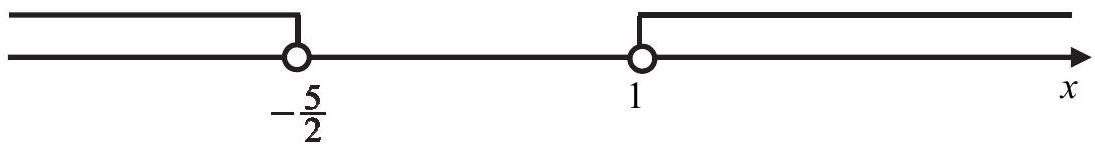
\includegraphics[max width=\textwidth, center]{2025_02_07_d6086222b99967346d9dg-09}
\end{itemize}

\section*{Kryteria uwzględniające specyficzne trudności w uczeniu się matematyki (dysleksja)}
Jeśli zdający pomyli porządek liczb na osi liczbowej, np. zapisze zbiór rozwiązań nierówności w postaci $(-\infty, 1) \cup\left(-\frac{5}{2},+\infty\right),\left(+\infty,-\frac{5}{2}\right) \cup(1,-\infty)$, to przyznajemy 2 punkty.

\section*{Uwagi}
\begin{enumerate}
  \item Akceptujemy zapisanie odpowiedzi w postaci: $x<-\frac{5}{2}$ i $x>1, x<-\frac{5}{2}$ oraz $x>1$.
  \item Jeżeli zdający dzieli obie strony nierówności przez $x-1$, rozważając dwa przypadki $x-1>0$ oraz $x-1<0$, rozwiąże nierówność $w$ każdym $z$ tych przypadków i poda zbiór rozwiązań każdej $z$ tych nierówności, to otrzymuje 2 punkty.
  \item Jeżeli zdający poprawnie obliczy pierwiastki trójmianu $x_{1}=-\frac{5}{2}, x_{2}=1$ i zapisze, np . $\left(-\infty,-\frac{5}{2}\right) \cup(-1,+\infty)$, popełniając tym samym błąd przy przepisywaniu jednego z pierwiastków, to otrzymuje 2 punkty.
  \item Jeżeli zdający poprawnie rozwiąże nierówność $2(x-1)(x+3)>x-1$, ale zapisze sprzeczną z tym rozwiązaniem odpowiedź, np. $x \notin R \backslash\left\{-\frac{5}{2}, 1\right\}$, albo $x \neq-\frac{5}{2}$ i $x \neq 1$, to otrzymuje 2 punkty.
  \item Jeżeli zdający rozwiązuje zadanie sposobem III i nie sprawdzi algebraicznie, że odczytane liczby $x_{1}=-\frac{5}{2}$ oraz $x_{2}=1$ są odciętymi punktów wspólnych wykresów funkcji $y=2(x-1)(x+3)$ oraz $y=x-1$, to otrzymuje 2 punkty.
  \item Jeżeli zdający pominie 2 w nierówności $2(x-1)(x+3)>x-1$ i rozwiąże nierówność $(x-1)(x+3)>x-1$, to może otrzymać co najwyżej 1 punkt za całe rozwiązanie.
  \item Jeżeli zdający rozwiązuje zadanie sposobem III i błędnie odczyta którąkolwiek z odciętych punktów wspólnych wykresów funkcji $y=2(x-1)(x+3)$ oraz $y=x-1$, to otrzymuje 1 punkt za całe rozwiązanie, pod warunkiem, że otrzyma sumę dwóch rozłącznych przedziałów otwartych.
  \item Jeżeli zdający podaje pierwiastki bez związku z trójmianem kwadratowym z zadania, to oznacza, że nie podjął realizacji pierwszego etapu rozwiązania i w konsekwencji otrzymuje $\mathbf{0}$ punktów za całe rozwiązanie.
  \item Jeżeli zdający wyznacza pierwiastki trójmianu kwadratowego w przypadku, gdy obliczony wyróżnik $\Delta$ jest niedodatni, to otrzymuje 0 punktów za całe rozwiązanie.
  \item Jeżeli zdający rozwiąże nierówność $2(x-1)(x+3)>0$, to otrzymuje $\mathbf{0}$ punktów za całe rozwiązanie.
  \item Jeżeli zdający dzieli obie strony nierówności przez $x-1$ bez stosownego założenia, to otrzymuje $\mathbf{0}$ punktów za całe rozwiązanie.
\end{enumerate}

\section*{Przykładowe rozwiązanie}
Pierwszy etap to wyznaczenie pierwiastków trójmianu kwadratowego: $2 x^{2}+3 x-5$.\\
Drugi etap to zapisanie zbioru rozwiązań nierówności kwadratowej.\\
Pierwszy etap rozwiązania może być realizowany następująco:

\section*{I sposób}
Przekształcamy równoważnie nierówność do postaci $(2 x+5)(x-1)>0$ (przenosimy wszystkie wyrażenia na lewą stronę nierówności i wyłączamy wspólny czynnik poza nawias), a następnie zapisujemy pierwiastki trójmianu $(2 x+5)(x-1): x_{1}=-\frac{5}{2}$ oraz $x_{2}=1$.

\section*{Il sposób}
Zapisujemy nierówność w postaci $2 x^{2}+3 x-5>0$ i obliczamy pierwiastki trójmianu\\
$2 x^{2}+3 x-5$

\begin{itemize}
  \item obliczamy wyróżnik tego trójmianu:
\end{itemize}

$$
\Delta=49 \text { i stąd } x_{1}=-\frac{5}{2} \text { oraz } x_{2}=1
$$

albo

\begin{itemize}
  \item stosujemy wzory Viète'a:\\
$x_{1} \cdot x_{2}=-\frac{5}{2}$ oraz $x_{1}+x_{2}=-\frac{3}{2}$, stąd $x_{1}=-\frac{5}{2}$ oraz $x_{2}=1$\\
albo
  \item podajemy je bezpośrednio, np. zapisując pierwiastki trójmianu lub postać iloczynowa trójmianu, lub zaznaczając je na wykresie (wystarczy szkic wykresu, oś liczbowa itp.): $x_{1}=-\frac{5}{2}$ oraz $x_{2}=1$ lub $2\left(x+\frac{5}{2}\right)(x-1)$.
\end{itemize}

\section*{Drugi etap rozwiązania:}
Zapisujemy zbiór rozwiązań nierówności: $\left(-\infty,-\frac{5}{2}\right) \cup(1,+\infty)$ lub $x \in\left(-\infty,-\frac{5}{2}\right) \cup(1,+\infty)$.

\section*{III sposób}
Wykonujemy rysunek pomocniczy. W jednym układzie współrzędnych szkicujemy fragment wykresu funkcji kwadratowej określonej wzorem $y=2(x-1)(x+3)$ oraz fragment wykresu funkcji liniowej określonej wzorem $y=x-1$.\\
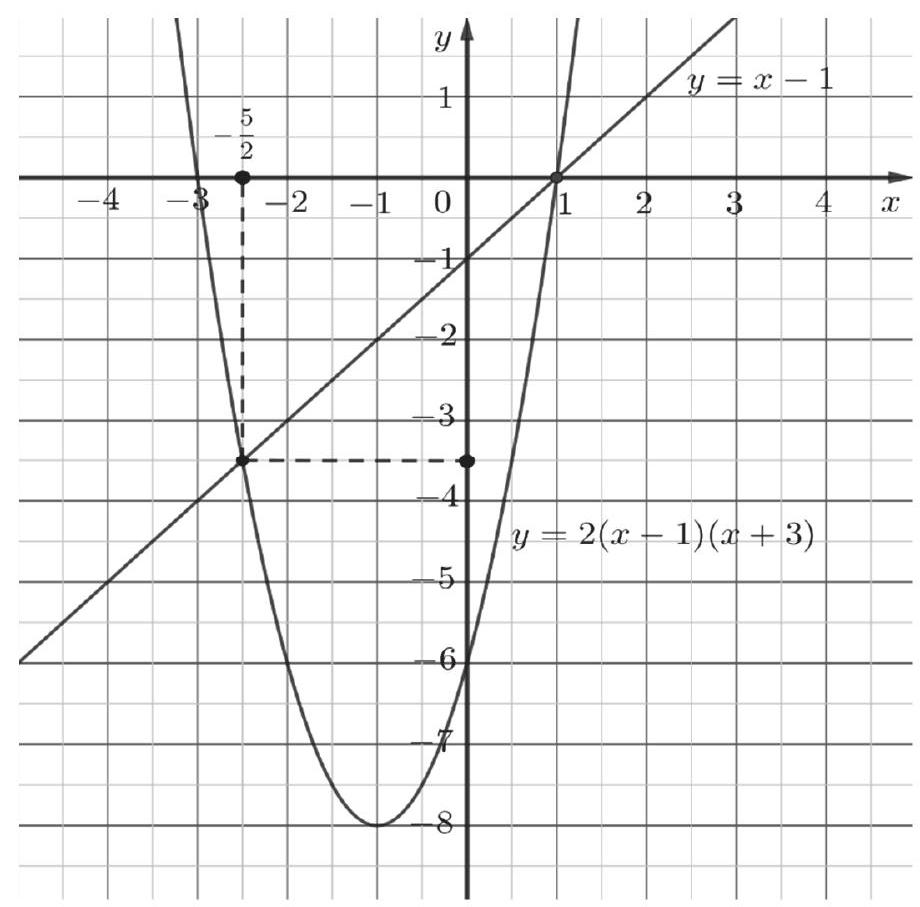
\includegraphics[max width=\textwidth, center]{2025_02_07_d6086222b99967346d9dg-11}

Odczytujemy odcięte punktów wspólnych obu wykresów. Są to liczby $x_{1}=-\frac{5}{2}$ oraz $x_{2}=1$. Sprawdzamy, czy odczytane współrzędne są odciętymi punktów wspólnych tych wykresów $2\left(-\frac{5}{2}-1\right)\left(-\frac{5}{2}+3\right)=2 \cdot\left(-\frac{7}{2}\right)\left(\frac{1}{2}\right)=-\frac{7}{2}$ $-\frac{5}{2}-1=-\frac{7}{2}$\\
Stąd liczba $\left(-\frac{5}{2}\right)$ jest odciętą punktu wspólnego obu wykresów, a liczba 1 jest wspólnym miejscem zerowym obu funkcji $y=2(x-1)(x+3)$ oraz $y=x-1$.\\
Z naszkicowanego wykresu odczytujemy te argumenty, dla których funkcja kwadratowa przyjmuje wartości większe niż funkcja liniowa $x \in\left(-\infty,-\frac{5}{2}\right) \cup(1,+\infty)$. Zatem zbiór ten jest zbiorem rozwiązań nierówności $2(x-1)(x+3)>x-1$.

\section*{Zadanie 27. (0-2)}
\begin{center}
\begin{tabular}{|l|l|}
\hline
\multicolumn{1}{|c|}{Wymaganie ogólne} & \multicolumn{1}{c|}{Wymaganie szczegółowe} \\
\hline
\begin{tabular}{l}
I. Wykorzystanie i tworzenie \\
informacji. \\
\end{tabular} & \begin{tabular}{l}
3. Równania i nierówności. Zdający korzysta \\
z własności iloczynu przy rozwiązywaniu równań \\
typu $x(x+1)(x-7)=0$ (3.7). \\
\end{tabular} \\
\hline
\end{tabular}
\end{center}

\section*{Zasady oceniania}
Zdający otrzymuje ........................................................................................................... 1 p.\\
gdy

\begin{itemize}
  \item zapisze dwa równania $x^{2}-1=0$ i $x^{2}-2 x=0$ lub z zapisu wynika, że rozwiązuje te równania\\
albo
  \item obliczy lub poda rozwiązania jednego z równań:\\
$x^{2}-1=0(x=1, x=-1)$ lub $x^{2}-2 x=0(x=0, x=2)$\\
i na tym zakończy lub dalej popełni błędy.
\end{itemize}

\section*{Zdający otrzymuje}
2 p.\\
gdy wyznaczy wszystkie rozwiązania równania: $x=0, x=2, x=1, x=-1$, ale nie uzyska ich w wyniku błędnej metody.

\section*{Uwagi}
\begin{enumerate}
  \item Jeżeli zdający poda wszystkie rozwiązania równania, bez zapisanych rachunków lub uzasadnienia, to otrzymuje 2 punkty.
  \item Jeżeli zdający poprawnie zapisze lewą stronę równania w postaci sumy jednomianów i doprowadzając ją do postaci iloczynu popełni błędy, ale skorzysta z własności iloczynu równego zero, to za całe rozwiązanie może otrzymać co najwyżej 1 punkt.
\end{enumerate}

\section*{Przykładowe rozwiązanie}
lloczyn jest równy zero, jeśli przynajmniej jeden z czynników jest równy zero.\\
Zatem $x^{2}-1=0$ lub $x^{2}-2 x=0$.\\
Równanie $x^{2}-1=0$ ma dwa rozwiązania: $x=-1$ lub $x=1$.\\
Równanie $x^{2}-2 x=0$ ma dwa rozwiązania: $x=0$ lub $x=2$.\\
Zatem rozwiązaniami równania $\left(x^{2}-1\right)\left(x^{2}-2 x\right)=0$ są liczby: $x=0, x=2, x=1, x=-1$.

\section*{Zadanie 28. (0-2)}
\begin{center}
\begin{tabular}{|c|c|}
\hline
Wymaganie ogólne & \multicolumn{1}{|c|}{Wymaganie szczegółowe} \\
\hline
V. Rozumowanie i argumentacja. & \begin{tabular}{l}
2. Wyrażenia algebraiczne. Zdający używa wzorów \\
skróconego mnożenia $(a \pm b)^{2}$ oraz $a^{2}-b^{2}(2.1)$. \\
\end{tabular} \\
\hline
\end{tabular}
\end{center}

\section*{Zasady oceniania I ill sposobu rozwiązania}
\section*{Zdajacy otrzymuje \\
 1 p. \\
 gdy}
\begin{itemize}
  \item zapisze nierówność w postaci $(a-b)^{2}+b^{2}>0$\\
albo
  \item obliczy wyróżnik trójmianu kwadratowego w zależności od zmiennej a lub $b$, występującego po jednej stronie nierówności, gdy po drugiej stronie jest 0 , i stwierdzi, że jest on niedodatni
\end{itemize}

\section*{albo}
\begin{itemize}
  \item obliczy wyróżnik trójmianu kwadratowego w zależności od zmiennej a lub $b$, występującego po jednej stronie nierówności, gdy po drugiej stronie jest 0 oraz rozważy jeden z przypadków $\Delta<0$ lub $\Delta=0$ i w tym przypadku doprowadzi rozumowanie do końca\\
i na tym zakończy lub dalej popełni błędy.
\end{itemize}

\section*{Zdający otrzymuje 2 p. gdy poda pełne uzasadnienie.}
\section*{Uwaga}
Jeżeli zdający sprawdza prawdziwość nierówności jedynie dla wybranych wartości a i $b$, to otrzymuje 0 punktów za całe rozwiązanie.

\section*{Zasady oceniania III sposobu rozwiązania \\
 Zdający otrzymuje}
gdy rozważy dwa przypadki:\\
w jednym, dla $a \neq 0$, podzieli stronami nierówność przez $a^{2}$, w drugim, dla $b \neq 0$, podzieli stronami nierówność przez $b^{2}$\\
i w jednym przypadku doprowadzi rozumowanie do końca.

\section*{Zdający otrzymuje}
2 p.\\
gdy zapisze pełne rozumowanie.

\section*{Uwaga}
Jeżeli zdający sprawdza prawdziwość nierówności jedynie dla wybranych wartości a i $b$, to otrzymuje 0 punktów za całe rozwiązanie.

\section*{Zasady oceniania IV sposobu rozwiązania \\
 Zdający otrzymuje \\
 1 p.}
gdy

\begin{itemize}
  \item rozważy trzy przypadki i zapisze nierówności $(a-\sqrt{2} b)^{2}>2 a b(1-\sqrt{2})$,
\end{itemize}

$$
(a+\sqrt{2} b)^{2}>2 a b(1+\sqrt{2}), a^{2}+2 b^{2}>0
$$

i na tym zakończy lub dalej popełni błędy.\\
albo

\begin{itemize}
  \item przeprowadzi pełne rozumowanie w dwóch spośród trzech przypadków i na tym zakończy lub dalej popełni błędy.\\
Zdający otrzymuje 2 p.\\
gdy zapisze pełne rozumowanie.
\end{itemize}

\section*{Uwaga}
Jeżeli zdający sprawdza prawdziwość nierówności jedynie dla wybranych wartości a i $b$, to otrzymuje 0 punktów za całe rozwiązanie.

\section*{Zasady oceniania V sposobu rozwiązania}
Zdający otrzymuje\\
1 p.\\
gdy przeprowadzając dowód nie wprost, zapisze nierówność $a(a-2 b)+2 b^{2} \leq 0$ w postaci $(a-b)^{2}+b^{2} \leq 0$\\
i na tym zakończy lub dalej popełni błędy.\\
Zdający otrzymuje 2 p. gdy zapisze pełne rozumowanie.

\section*{Uwaga}
Jeżeli zdający sprawdza prawdziwość nierówności jedynie dla wybranych wartości a i $b$, to otrzymuje $\mathbf{0}$ punktów za całe rozwiązanie.

\section*{Zasady oceniania VI sposobu rozwiązania}
Zdający otrzymuje\\
gdy zapisze nierówność w postaci równoważnej $a^{2}+2 b^{2}>2 a b$ oraz zapisze, że dla dowolnych liczb rzeczywistych $a, b$ prawdziwe są nierówności:

$$
a^{2}+2 b^{2} \geq a^{2}+b^{2} \text { oraz } a^{2}+b^{2} \geq 2 a b
$$

i na tym zakończy lub dalej popełni błędy\\
Zdający otrzymuje\\
2 p. gdy zapisze pełne rozumowanie.

\section*{Uwaga}
Jeżeli zdający sprawdza prawdziwość nierówności jedynie dla wybranych wartości a i $b$, to otrzymuje $\mathbf{0}$ punktów za całe rozwiązanie.

\section*{Przykładowe rozwiązania}
\section*{I sposób}
Przekształcamy równoważnie nierówność i otrzymujemy kolejno:

$$
\begin{gathered}
a^{2}-2 a b+2 b^{2}>0, \\
a^{2}-2 a b+b^{2}+b^{2}>0, \\
(a-b)^{2}+b^{2}>0
\end{gathered}
$$

Nierówność $(a-b)^{2}+b^{2}>0$ jest prawdziwa, ponieważ:

\begin{enumerate}
  \item wyrażenie $(a-b)^{2}$ jest dodatnie, gdyż z założenia wynika $a-b \neq 0$ i kwadrat każdej liczby rzeczywistej różnej od zera jest dodatni,
  \item wyrażenie $b^{2}$ jest nieujemne,
  \item suma dwóch liczb rzeczywistych, z których jedna jest liczbą dodatnią, a druga liczbą nieujemna, jest liczbą dodatnią.
\end{enumerate}

\section*{To kończy dowód.}
\section*{Il sposób}
Przekształcamy równoważnie nierówność i otrzymujemy:

$$
a^{2}-2 a b+2 b^{2}>0
$$

Wyrażenie $a^{2}-2 a b+2 b^{2}$ traktujemy jako trójmian kwadratowy jednej zmiennej np. a.\\
Wyróżnik trójmianu kwadratowego $a^{2}-2 a b+2 b^{2}$ jest równy: $\Delta=4 b^{2}-8 b^{2}=-4 b^{2}$.\\
Ten wyróżnik jest niedodatni dla każdej rzeczywistej wartości $b$.\\
Gdy $\Delta<0$, to $a^{2}-2 a b+2 b^{2}>0$ dla każdej rzeczywistej wartości $a$.\\
Gdy $\Delta=0$, to $b=0$, stąd $a^{2}>0$, ponieważ z założenia $a \neq b$.\\
Oznacza to, że dla każdych dwóch różnych liczb rzeczywistych a i b prawdziwa jest nierówność $a^{2}-2 a b+2 b^{2}>0$.

\section*{To kończy dowód.}
\section*{Ill sposób}
Przekształcamy równoważnie nierówność $a(a-2 b)+2 b^{2}>0$ i otrzymujemy:

$$
a^{2}-2 a b+2 b^{2}>0
$$

Z założenia wynika, że liczby $a$ i $b$ nie mogą jednocześnie przyjmować wartości 0 .\\
Jeżeli $b \neq 0$, to $b^{2}>0$. Dzielimy obie strony nierówności przez $b^{2}$ i otrzymujemy nierówność równoważną

$$
\left(\frac{a}{b}\right)^{2}-2 \frac{a}{b}+2>0
$$

Niech $x=\frac{a}{b}$. Otrzymujemy nierówność kwadratową $x^{2}-2 x+2>0 \quad z$ niewiadomą $x$. Zauważamy, że ta nierówność jest prawdziwa dla każdej liczby rzeczywistej $x$, bo z równości

$$
x^{2}-2 x+2=(x-1)^{2}+1
$$

wnioskujemy, że $(x-1)^{2}+1>0$, wobec oczywistej nierówności $(x-1)^{2} \geq 0$.

Natomiast jeżeli $a \neq 0$, to $a^{2}>0$. Dzielimy obie strony nierówności przez $a^{2}$ i otrzymujemy nierówność równoważną

$$
2\left(\frac{b}{a}\right)^{2}-2 \frac{b}{a}+1>0 .
$$

Niech teraz $x=\frac{b}{a}$. Otrzymujemy nierówność kwadratową $2 x^{2}-2 x+1>0$ z niewiadomą $x$.\\
Ponieważ wyróżnik trójmianu $2 x^{2}-2 x+1$ jest ujemny oraz współczynnik przy najwyższej potędze trójmianu jest dodatni, więc ten trójmian przyjmuje tylko wartości dodatnie dla każdej liczby rzeczywistej $x$.\\
Z rozważonych przypadków wynika, że nierówność jest prawdziwa dla każdych dwóch różnych liczb rzeczywistych a i $b$.

\section*{To kończy dowód.}
\section*{IV sposób}
Niech $a \neq b$. Rozważmy następujące przypadki:\\
Przypadek I: $a \cdot b>0$.\\
Przekształcamy równoważnie nierówność $a(a-2 b)+2 b^{2}>0$ i otrzymujemy:

$$
a^{2}+2 b^{2}-2 \sqrt{2} a b>2 a b-2 \sqrt{2} a b .
$$

Stąd $(a-\sqrt{2} b)^{2}>2 a b(1-\sqrt{2})$.\\
Wyrażenie $(a-\sqrt{2} b)^{2}$ jest nieujemne. Wyrażenie $2 a b(1-\sqrt{2})$ jest ujemne, ponieważ $1-\sqrt{2}<0$ i z założenia $a b>0$.

Nierówność jest prawdziwa dla każdych dwóch liczb rzeczywistych a i $b$, takich, że $a \cdot b>0$ i $a \neq b$.

Przypadek II: $a \cdot b<0$.\\
Przekształcamy równoważnie nierówność $a(a-2 b)+2 b^{2}>0$ i otrzymujemy:

$$
a^{2}+2 b^{2}+2 \sqrt{2} a b>2 a b+2 \sqrt{2} a b .
$$

Stąd $(a+\sqrt{2} b)^{2}>2 a b(1+\sqrt{2})$.\\
Wyrażenie $(a+\sqrt{2} b)^{2}$ jest nieujemne. Wyrażenie $2 a b(1+\sqrt{2})$ jest ujemne, ponieważ $1+\sqrt{2}>0$ i z założenia $a b<0$.

Nierówność jest prawdziwa dla każdych dwóch liczb rzeczywistych a i b, takich, że $a \cdot b<0$ i $a \neq b$.

Przypadek III: $a \cdot b=0$\\
Przekształcamy równoważnie nierówność $a(a-2 b)+2 b^{2}>0$ i otrzymujemy:

$$
a^{2}-2 a b+2 b^{2}>0 .
$$

Ponieważ $a \cdot b=0$, więc nierówność $a^{2}-2 a b+2 b^{2}>0$ możemy zapisać w postaci $a^{2}+2 b^{2}>0$.

Suma kwadratów dwóch dowolnych liczb rzeczywistych a i $b$, takich, że $a \neq b$ jest dodatnia.\\
Nierówność jest prawdziwa dla każdych dwóch liczb rzeczywistych a i $b$, takich, że $a \cdot b=0$ i $a \neq b$.

\section*{To kończy dowód.}
$\underline{\text { V sposób }}$ (dowód nie wprost)\\
Załóżmy, że istnieją różne liczby rzeczywiste a i $b$, dla których prawdziwa jest nierówność

$$
a(a-2 b)+2 b^{2} \leq 0
$$

Powyższa nierówność jest równoważna nierównościom:

$$
\begin{gathered}
a^{2}-2 a b+2 b^{2} \leq 0 \\
(a-b)^{2}+b^{2} \leq 0
\end{gathered}
$$

Ponieważ lewa strona tej nierówności jest sumą dwóch liczb nieujemnych $(a-b)^{2}$ i $b^{2}$, więc może zachodzić jedynie przypadek $(a-b)^{2}+b^{2}=0$. Wynika stąd, że $a-b=0$ i $b=0$. Zatem $a=0$ i $b=0$, co przeczy założeniu, że liczby a i $b$ są różne.\\
Otrzymana sprzeczność oznacza, że nierówność $a(a-2 b)+2 b^{2} \leq 0$ jest fałszywa.\\
Prawdziwa zatem jest nierówność $a(a-2 b)+2 b^{2}>0$, dla każdych dwóch różnych liczb rzeczywistych a i $b$.

\section*{To kończy dowód.}
\section*{VI sposób (szacowanie)}
Nierówność $a(a-2 b)+2 b^{2}>0$ jest równoważna nierówności $a^{2}+2 b^{2}>2 a b$.\\
Dla dowolnych liczb rzeczywistych $a, b$ prawdziwe są nierówności $a^{2}+2 b^{2} \geq a^{2}+b^{2}$ oraz $a^{2}+b^{2} \geq 2 a b$, przy czym $a^{2}+b^{2}=2 a b$ tylko wtedy, gdy $a=b$. Ale z założenia $a \neq b$, więc otrzymujemy $a^{2}+2 b^{2} \geq a^{2}+b^{2}>2 a b$.

To kończy dowód.

\section*{Zadanie 29. (0-2)}
\begin{center}
\begin{tabular}{|l|l|}
\hline
\multicolumn{1}{|c|}{Wymaganie ogólne} & \multicolumn{1}{c|}{Wymaganie szczegółowe} \\
\hline
V. Rozumowanie i argumentacja. & \begin{tabular}{l}
7. Planimetria. Zdajacy rozpoznaje trójkaty podobne \\
i wykorzystuje (także w kontekstach praktycznych) \\
cechy podobieństwa trójkątów (7.1). \\
SP9. Wielokáty, koła, okręgi. Zdajacy rozpoznaje \\
i nazywa trójkąty ostrokatne, prostokątne \\
i rozwartokątne, równoboczne i równoramienne \\
(SP9.1). \\
\end{tabular} \\
\hline
\end{tabular}
\end{center}

\section*{Zasady oceniania}
Zdający otrzymuje

\begin{itemize}
  \item wyznaczy długości odcinków BC i CF w zależności od tej samej zmiennej, np.: $|B C|=a$
\end{itemize}

$$
\text { i }|C F|=\frac{3 \sqrt{3} a}{8} \cdot \frac{\sqrt{3}}{2} \text { lub }|B C|=2 x \text { i }|C F|=\frac{9}{8} x
$$

albo

\begin{itemize}
  \item wyznaczy skalę podobieństwa trójkątów $B C D$ i $C E F: k=\frac{8 \sqrt{3}}{9}$\\
albo
  \item wyznaczy długość odcinka CF w zależności od długości odcinków CB i CD oraz\\
zależność między długościami odcinków $C D$ i $C B$, np.: $|C F|=\frac{3|C D|^{2}}{4|C B|},|C D|=\frac{\sqrt{3}}{2}|C B|$\\
i na tym poprzestanie lub dalej popełni błędy.\\
Zdający otrzymuje 2 p. gdy zapisze pełne rozumowanie.
\end{itemize}

\section*{Uwaga}
Ponieważ podobieństwo zachowuje stosunek długości odcinków, więc jeżeli zdający przyjmuje konkretną wartość długości boku trójkąta i przeprowadzi rozumowanie do końca, ale nie odwołuje się do tej własności, to może otrzymać co najwyżej 1 punkt.

\section*{Przykładowe rozwiązania}
\section*{I sposób}
\begin{center}
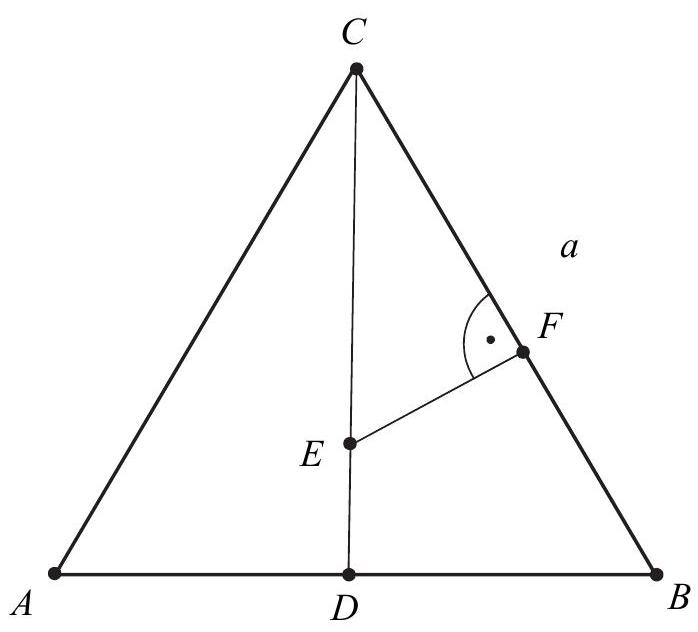
\includegraphics[max width=\textwidth]{2025_02_07_d6086222b99967346d9dg-19}
\end{center}

Niech $|B C|=a$. Wtedy $|C D|=\frac{a \sqrt{3}}{2}$. Ponieważ $|C E|=\frac{3}{4}|C D|$, to $|C E|=\frac{3 \sqrt{3} a}{8}$.\\
Zatem $|C F|=|C E| \cdot \frac{\sqrt{3}}{2}=\frac{3 \sqrt{3} a}{8} \cdot \frac{\sqrt{3}}{2}=\frac{9}{16} a=\frac{9}{16}|B C|$.

\section*{To kończy dowód.}
\section*{Il sposób}
\begin{center}
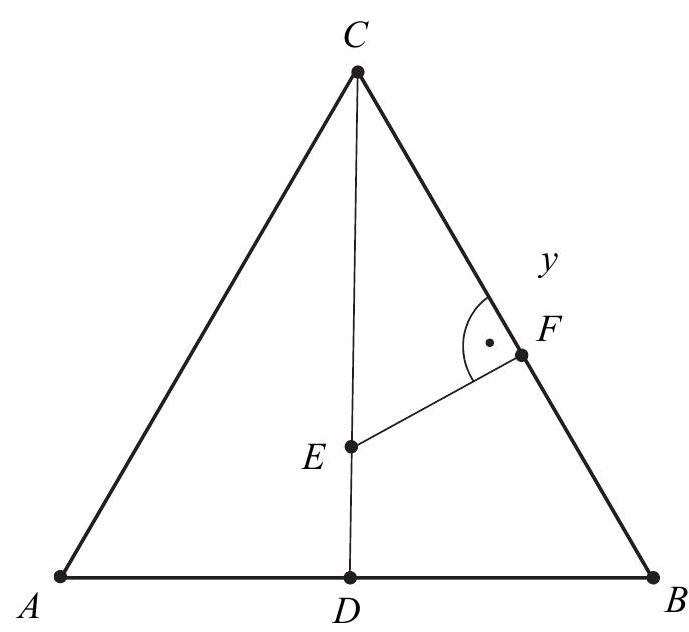
\includegraphics[max width=\textwidth]{2025_02_07_d6086222b99967346d9dg-19(1)}
\end{center}

Trójkąt $B C D$ jest trójkątem prostokątnym o kątach ostrych $30^{\circ}$ i $60^{\circ}$. Niech $|B C|=y$.\\
Wtedy $|C D|=\frac{y \sqrt{3}}{2}$. Trójkąt CEF jest połową trójkąta równobocznego. Niech $|C F|=x$. Stąd $|C E|=\frac{2 x \sqrt{3}}{3}$. Ponieważ $|C E|=\frac{3}{4}|C D|$, to $\frac{2 x \sqrt{3}}{3}=\frac{3}{4} \cdot \frac{y \sqrt{3}}{2}$. Stąd $x=\frac{9}{16} y$.

To kończy dowód.

\section*{Ill sposób}
\begin{center}
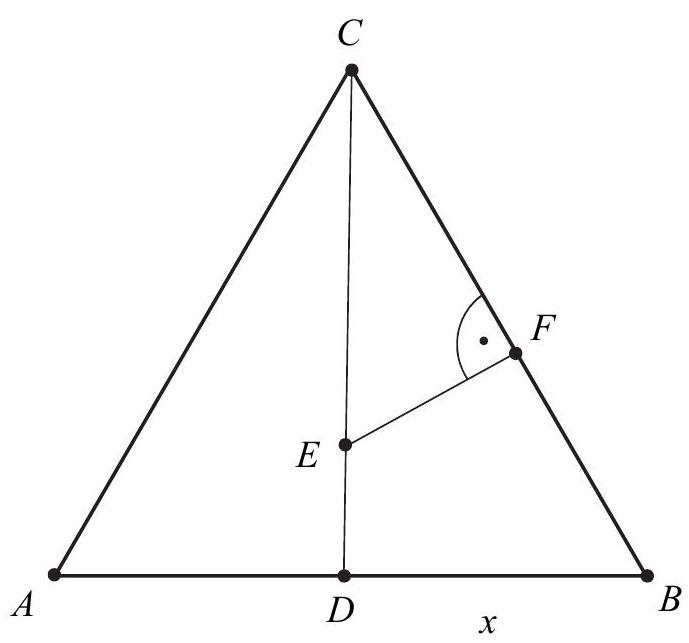
\includegraphics[max width=\textwidth]{2025_02_07_d6086222b99967346d9dg-20}
\end{center}

Niech $x=|B D|$. Trójkąt $B C D$ jest trójkątem prostokątnym o kątach ostrych $30^{\circ}$ i $60^{\circ}$, więc

$$
|B C|=2 x \text { oraz }|C D|=x \sqrt{3} .
$$

Ponieważ $|C E|=\frac{3}{4}|C D|$, więc $|C E|=\frac{3}{4} x \sqrt{3}$. Trójkąt $C E F$ jest połową trójkąta równobocznego,\\
więc $|C F|=\frac{\frac{3}{4} x \sqrt{3} \cdot \sqrt{3}}{2}=\frac{9}{8} x$.\\
Stąd $\frac{|C F|}{|C B|}=\frac{\frac{9}{8} x}{2 x}=\frac{9}{16}$. Zatem $|C F|=\frac{9}{16}|C B|$.

\section*{To kończy dowód.}
\section*{IV sposób}
\begin{center}
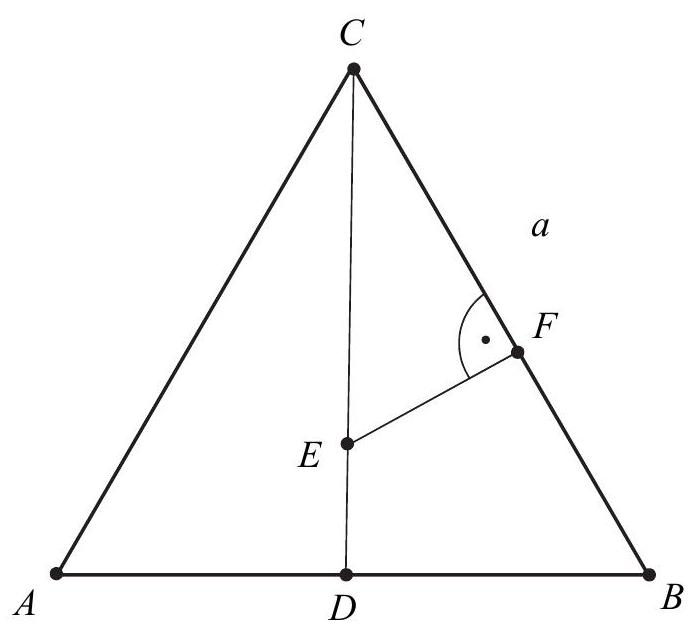
\includegraphics[max width=\textwidth]{2025_02_07_d6086222b99967346d9dg-20(1)}
\end{center}

Trójkąty BCD i ECF są podobne na podstawie cechy (kąt, kąt, kąt). Przyjmijmy następujące oznaczenie: $|B C|=a$, wtedy $|C D|=h=\frac{a \sqrt{3}}{2}$. Skalę podobieństwa można obliczyć w następujący sposób:\\
$k=\frac{|B C|}{|C E|}=\frac{a}{\frac{3}{4} h}=\frac{a}{\frac{3}{4} \cdot \frac{a \sqrt{3}}{2}}=\frac{8 \sqrt{3}}{9}$ oraz $k=\frac{|C D|}{|C F|}$.\\
Stąd $|C F|=\frac{|C D|}{k}=\frac{a \sqrt{3}}{2} \cdot \frac{9}{8 \sqrt{3}}=\frac{9}{16} a$.\\
To kończy dowód.

\section*{Zadanie 30. (0-2)}
\begin{center}
\begin{tabular}{|c|l|}
\hline
\multicolumn{1}{|c|}{Wymaganie ogólne} & \multicolumn{1}{c|}{Wymaganie szczegółowe} \\
\hline
III. Modelowanie matematyczne. & \begin{tabular}{l}
10. Elementy statystyki opisowej. Teoria \\
prawdopodobieństwa i kombinatoryka. Zdający \\
oblicza prawdopodobieństwa w prostych sytuacjach, \\
stosujacc klasyczną definicję prawdopodobieństwa \\
(10.3). \\
\end{tabular} \\
\hline
\end{tabular}
\end{center}

\section*{Zasady oceniania}
Zdający otrzymuje 1 p.\\
gdy

\begin{itemize}
  \item zapisze liczbę wszystkich zdarzeń elementarnych $|\Omega|=6^{2}=36$ lub opisze zbiór zdarzeń elementarnych za pomocą tabeli\\
albo
  \item wypisze wszystkie zdarzenia elementarne sprzyjające zdarzeniu $A$ :\\
$A=\{(1,5),(2,5),(3,5),(4,5),(5,5),(5,6),(5,1),(5,2),(5,3),(5,4),(6,5)\}$\\
lub zaznaczy je wszystkie w tabeli lub zaznaczy wszystkie istotne gałęzie na pełnym drzewie składającym się z 36 gałęzi,\\
albo
  \item obliczy liczbę zdarzeń elementarnych sprzyjających zdarzeniu $A$, np.: $|A|=2 \cdot 6-1=11$, $|A|=5+5+1=11$ i nie wskaże przy tym niepoprawnych zdarzeń elementarnych sprzyjających zdarzeniu $A$,\\
albo
  \item zapisze prawdopodobieństwa potrzebne do wyznaczenia końcowego wyniku na dwóch etapach (przy stosowaniu metody drzewa probabilistycznego składającego się z czterech gałęzi) oraz wskaże wszystkie istotne gałęzie (dla zdarzenia A lub zdarzenia $A^{\prime}$ )\\
i na tym zakończy lub dalej popełni błędy.\\
Zdający otrzymuje\\
gdy obliczy prawdopodobieństwo zdarzenia $A: P(A)=\frac{|A|}{|\Omega|}=\frac{11}{36}$.
\end{itemize}

\section*{Uwagi}
\begin{enumerate}
  \item Jeżeli zdający zapisze tylko: $|A|=11,|\Omega|=36, P(A)=\frac{11}{36}$, lub zapisze tylko: $P(A)=\frac{11}{36}$, lub $\frac{11}{36}$, to otrzymuje 2 punkty.
  \item Jeżeli zdający zapisze prawdopodobieństwo $P(A)=\frac{1}{6} \cdot \frac{1}{6}+2 \cdot \frac{1}{6} \cdot \frac{5}{6}$, to otrzymuje 2 punkty.
  \item Jeżeli zdający zapisze tylko $|A|=11$, to otrzymuje 1 punkt.
  \item Jeżeli zdający popełni błąd przy wypisywaniu zdarzeń elementarnych i wypisze o jedno za mało lub jedno powtórzy, ale nie wypisze żadnego niewłaściwego i konsekwentnie do popełnionego błędu obliczy prawdopodobieństwo, to otrzymuje 1 punkt.
  \item Jeżeli zdający stosuje drzewo probabilistyczne o 36 gałęziach, w którym przynajmniej 7 gałęzi odpowiada sytuacjom sprzyjającym rozważanemu zdarzeniu A (lub przynajmniej 13, gdy rozpatruje zdarzenie $A^{\prime}$ ), ale nie wskaże gałęzi niewłaściwej, i konsekwentnie do popełnionego błędu obliczy prawdopodobieństwo, to otrzymuje 1 punkt.
  \item Jeżeli zdający narysuje tylko drzewko i nie zaznaczy oraz nie opisze żadnej gałęzi, to otrzymuje 0 punków.
  \item Jeżeli zdający zapisze tylko liczby 36 lub 11 lub 25 i z rozwiązania zadania nie wynika znaczenie tych liczb, to otrzymuje 0 punktów.
  \item Jeśli zdający rozwiąże zadanie do końca i otrzyma $P(A)>1$ lub $\quad P(A)<0$, to otrzymuje za całe rozwiązanie 0 punktów, o ile końcowy wynik nie jest skutkiem błędu w działaniach na ułamkach.
\end{enumerate}

\section*{Przykładowe rozwiązania}
\section*{I sposób}
Obliczamy liczbę wszystkich zdarzeń elementarnych tego doświadczenia $|\Omega|=6^{2}=36$ lub opisujemy zbiór zdarzeń elementarnych np. w postaci tabeli

\begin{center}
\begin{tabular}{|c|c|c|c|c|c|c|}
\hline
 & $\mathbf{1}$ & $\mathbf{2}$ & $\mathbf{3}$ & $\mathbf{4}$ & $\mathbf{5}$ & $\mathbf{6}$ \\
\hline
$\mathbf{1}$ & $(1,1)$ & $(1,2)$ & $(1,3)$ & $(1,4)$ & $\mathbf{( 1 , 5 )}$ & $(1,6)$ \\
\hline
$\mathbf{2}$ & $(2,1)$ & $(2,2)$ & $(2,3)$ & $(2,4)$ & $(2,5)$ & $(2,6)$ \\
\hline
$\mathbf{3}$ & $(3,1)$ & $(3,2)$ & $(3,3)$ & $(3,4)$ & $(3,5)$ & $(3,6)$ \\
\hline
$\mathbf{4}$ & $(4,1)$ & $(4,2)$ & $(4,3)$ & $(4,4)$ & $\mathbf{( 4 , 5 )}$ & $(4,6)$ \\
\hline
$\mathbf{5}$ & $(5,1)$ & $(5,2)$ & $(5,3)$ & $(5,4)$ & $\mathbf{( 5 , 5 )}$ & $(5,6)$ \\
\hline
$\mathbf{6}$ & $(6,1)$ & $(6,2)$ & $(6,3)$ & $(6,4)$ & $\mathbf{( 6 , 5 )}$ & $(6,6)$ \\
\hline
\end{tabular}
\end{center}

Wskazujemy elementy zbioru A i zliczamy je:

$$
|A|=11 .
$$

Obliczamy prawdopodobieństwo zdarzenia A. Ponieważ wszystkie zdarzenia jednoelementowe są jednakowo prawdopodobne, więc korzystamy z klasycznej definicji prawdopodobieństwa:

$$
P(A)=\frac{|A|}{|\Omega|}=\frac{11}{36} .
$$

\section*{Il sposób}
Obliczamy liczbę wszystkich zdarzeń elementarnych: $|\Omega|=6^{2}=36$.\\
A - zdarzenie polegające na tym, że co najmniej jeden raz wypadnie ścianka z pięcioma oczkami.\\
$A^{\prime}$ - zdarzenie polegające na tym, że ani razu nie wypadnie ścianka z pięcioma oczkami.\\
Wskazujemy elementy zbioru $A^{\prime}$ (wypisujemy lub zaznaczamy w tabeli) i zliczamy je:

\begin{center}
\begin{tabular}{|c|c|c|c|c|c|c|}
\hline
 & $\mathbf{1}$ & $\mathbf{2}$ & $\mathbf{3}$ & $\mathbf{4}$ & $\mathbf{5}$ & $\mathbf{6}$ \\
\hline
$\mathbf{1}$ & $\mathbf{( 1 , 1 )}$ & $\mathbf{( 1 , 2 )}$ & $(1,3)$ & $\mathbf{( 1 , 4 )}$ & $(1,5)$ & $(1,6)$ \\
\hline
$\mathbf{2}$ & $(\mathbf{( 2 , 1 )}$ & $(2,2)$ & $(2,3)$ & $(2,4)$ & $(2,5)$ & $(\mathbf{( 2 , 6 )}$ \\
\hline
$\mathbf{3}$ & $(3,1)$ & $(3,2)$ & $(3,3)$ & $(3,4)$ & $(3,5)$ & $(3,6)$ \\
\hline
$\mathbf{4}$ & $\mathbf{( 4 , 1 )}$ & $\mathbf{( 4 , 2 )}$ & $(4,3)$ & $(4,4)$ & $(4,5)$ & $\mathbf{( 4 , 6 )}$ \\
\hline
$\mathbf{5}$ & $(5,1)$ & $(5,2)$ & $(5,3)$ & $(5,4)$ & $(5,5)$ & $(5,6)$ \\
\hline
$\mathbf{6}$ & $\mathbf{( 6 , 1 )}$ & $\mathbf{( 6 , 2 )}$ & $\mathbf{( 6 , 3 )}$ & $\mathbf{( 6 , 4 )}$ & $(6,5)$ & $\mathbf{( 6 , 6 )}$ \\
\hline
\end{tabular}
\end{center}

$$
\left|A^{\prime}\right|=5^{2}=25 .
$$

Obliczamy prawdopodobieństwo zdarzenia A: $P(A)=1-P\left(A^{\prime}\right)=1-\frac{25}{36}=\frac{11}{36}$.

\section*{III sposób (metoda drzewka)}
Przedstawiamy model graficzny doświadczenia.\\
5 - oznacza wypadnięcie ścianki kostki z pięcioma oczkami, z - oznacza wypadnięcie innej ścianki niż z pięcioma oczkami.\\
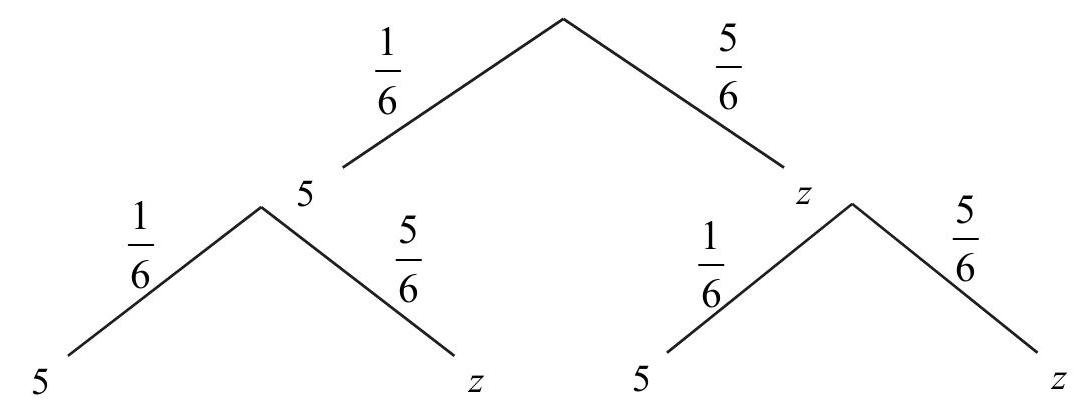
\includegraphics[max width=\textwidth, center]{2025_02_07_d6086222b99967346d9dg-23}

Prawdopodobieństwo zdarzenia $A$ jest równe: $P(A)=\frac{1}{6} \cdot \frac{1}{6}+\frac{1}{6} \cdot \frac{5}{6}+\frac{5}{6} \cdot \frac{1}{6}=\frac{11}{36}$.\\
Zadanie 31. (0-2)

\begin{center}
\begin{tabular}{|l|l|}
\hline
\multicolumn{1}{|c|}{Wymaganie ogólne} & \multicolumn{1}{c|}{Wymaganie szczegółowe} \\
\hline
IV. Użycie i tworzenie strategii. & \begin{tabular}{l}
6. Trygonometria. Zdający stosuje proste zależności \\
między funkcjami trygonometrycznymi: \\
 \\
 \\
 \\
$\sin ^{2} \alpha+\cos ^{2} \alpha=1, \operatorname{tg} \alpha=\frac{\sin \alpha}{\cos \alpha}$, oraz \\
$\sin \left(90^{\circ}-\alpha\right)=\cos \alpha(6.4)$. \\
\end{tabular} \\
\hline
\end{tabular}
\end{center}

\section*{Zasady oceniania I, II, III i IV sposobu rozwiązania}
Zdający otrzymuje\\
gdy przekształci równanie $\frac{2 \sin \alpha+3 \cos \alpha}{\cos \alpha}=4$ do postaci:\\
$2 \operatorname{tg} \alpha+3=4$ lub $2 \sin \alpha=\cos \alpha$ lub $2 \sin \alpha-\cos \alpha=0$ lub $2 \frac{a}{c}=\frac{b}{c}$ lub $2 a=b$\\
i na tym zakończy lub dalej popełni błędy.\\
Zdający otrzymuje 2 p.\\
gdy obliczy tangens kąta $\alpha: \operatorname{tg} \alpha=\frac{1}{2}$, ale nie uzyska go w wyniku błędnej metody.

\section*{Uwagi}
\begin{enumerate}
  \item Jeżeli zdający popełni błąd i zapisze $\operatorname{tg} \alpha=\frac{\cos \alpha}{\sin \alpha}$, to otrzymuje co najwyżej 1 punkt za całe rozwiązanie.
  \item Jeżeli zdający popełni jedyny błąd polegający na zastosowaniu niepoprawnego wzoru $\sqrt{a-b}=\sqrt{a}-\sqrt{b}$ albo $(a+b)^{2}=a^{2}+b^{2}$ i konsekwentnie doprowadzi rozwiązanie do końca, to może otrzymać za całe rozwiązanie co najwyżej 1 punkt.
\end{enumerate}

\section*{Przykładowe rozwiązania}
\section*{I sposób}
Równanie $\frac{2 \sin \alpha+3 \cos \alpha}{\cos \alpha}=4$ przekształcamy równoważnie do postaci:

$$
\frac{2 \sin \alpha}{\cos \alpha}+\frac{3 \cos \alpha}{\cos \alpha}=4
$$

Stąd $2 \operatorname{tg} \alpha+3=4$, czyli $\operatorname{tg} \alpha=\frac{1}{2}$.

\section*{II sposób}
Równanie $\frac{2 \sin \alpha+3 \cos \alpha}{\cos \alpha}=4$ przekształcamy równoważnie do postaci:

$$
2 \sin \alpha+3 \cos \alpha=4 \cos \alpha
$$

Stąd $2 \sin \alpha=\cos \alpha$, czyli $\operatorname{tg} \alpha=\frac{1}{2}$.

\section*{III sposób}
Rysujemy trójkąt prostokątny, w którym oznaczamy długości przyprostokątnych a i $b$, długość przeciwprostokątnej coraz zaznaczamy kąt ostry $\alpha$ taki, że $\sin \alpha=\frac{a}{c}$ lub $\cos \alpha=\frac{b}{c}$.\\
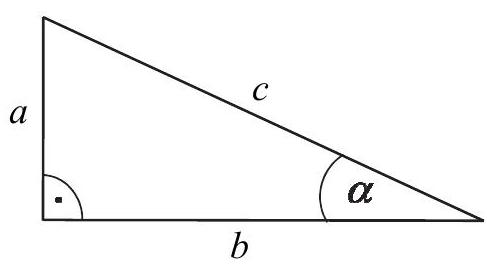
\includegraphics[max width=\textwidth, center]{2025_02_07_d6086222b99967346d9dg-25}

Podane równanie $\frac{2 \sin \alpha+3 \cos \alpha}{\cos \alpha}=4$ zapisujemy w postaci $\frac{2 \cdot \frac{a}{c}+3 \cdot \frac{b}{c}}{\frac{b}{c}}=4$. Następnie wykonujemy przekształcenia na lewej stronie tej równości i otrzymujemy $\frac{2 a+3 b}{b}=4$. Stąd wynika, że $2 a+3 b=4 b$, czyli $2 a=b$. Ostatnia równość oznacza, że $\frac{a}{b}=\frac{1}{2}$. Zatem $\operatorname{tg} \alpha=\frac{1}{2}$.

\section*{IV sposób}
Równanie $\frac{2 \sin \alpha+3 \cos \alpha}{\cos \alpha}=4$ przekształcamy równoważnie do postaci

$$
2 \sin \alpha+3 \cos \alpha=4 \cos \alpha
$$

Stąd wynika, że $2 \sin \alpha=\cos \alpha$. Korzystamy z tożsamości $\sin ^{2} \alpha+\cos ^{2} \alpha=1$ i otrzymujemy równanie $\sin ^{2} \alpha+(2 \sin \alpha)^{2}=1$. Stąd $\sin ^{2} \alpha=\frac{1}{5}$. Ponieważ $\alpha$ jest kątem ostrym, więc $\sin \alpha=\frac{1}{\sqrt{5}}$.\\
Ale $\cos \alpha=2 \sin \alpha$, więc $\cos \alpha=\frac{2}{\sqrt{5}}$. Ostatecznie $\operatorname{tg} \alpha=\frac{\sin \alpha}{\cos \alpha}=\frac{\frac{1}{\sqrt{5}}}{\frac{2}{\sqrt{5}}}=\frac{1}{2}$.

\section*{Zadanie 32. (0-4)}
\begin{center}
\begin{tabular}{|l|l|}
\hline
\multicolumn{1}{|c|}{Wymaganie ogólne} & \multicolumn{1}{c|}{Wymaganie szczegółowe} \\
\hline
IV. Użycie i tworzenie strategii. & \begin{tabular}{l}
8. Geometria na płaszczyźnie kartezjańskiej. Zdajacy \\
wyznacza równanie prostej, która jest równoległa lub \\
prostopadła do prostej danej w postaci kierunkowej \\
i przechodzi przez dany punkt (8.3). Zdający oblicza \\
wspórzędne punktu przecięcia dwóch prostych (8.4). \\
Zdajacy wyznacza współrzędne środka odcinka \\
(8.5). \\
\end{tabular} \\
\hline
\end{tabular}
\end{center}

\section*{Zasady oceniania I, II, III i IV sposobu rozwiązania}
Rozwiązanie, w którym postęp jest niewielki, ale konieczny na drodze do pełnego rozwiązania\\
Zdający

\begin{itemize}
  \item wyznaczy równanie prostej $A C: y=-\frac{3}{4} x+\frac{25}{12}$\\
albo
  \item obliczy odległość punktu $A$ od prostej $B D: 5$\\
albo
  \item zapisze współrzędne punktu $P$ leżącego na prostej o równaniu $y=\frac{4}{3} x$, np. $P=\left(x, \frac{4}{3} x\right)$ i wyznaczy odległość punktu $P$ od danego punktu $A$ jako funkcję jednej zmiennej $x:|A P|=\sqrt{(x-5)^{2}+\left(\frac{4}{3} x+\frac{5}{3}\right)^{2}}$\\
albo\\
wyznaczy równania prostych $A B$ i $A D$ : $y+\frac{5}{3}=\frac{1}{7}(x-5)$ oraz $y+\frac{5}{3}=-7(x-5)$,\\
i na tym zakończy lub dalej popełni błędy.\\
Rozwiązanie, w którym jest istotny postęp\\
2 p.\\
Zdający
  \item wyznaczy równanie prostej $A C$ : $y=-\frac{3}{4} x+\frac{25}{12}$ i obliczy współrzędne punktu przecięcia przekątnych kwadratu: $O=\left(1, \frac{4}{3}\right)$\\
albo
  \item obliczy odległość punktu $A$ od prostej $B D$ : 5 i obliczy pole kwadratu: 50\\
albo
  \item obliczy odległość punktu $A$ od prostej $B D: 5$ i zapisze równanie $\left(x_{o}-5\right)^{2}+\left(\frac{4}{3} x_{o}+\frac{5}{3}\right)^{2}=25$\\
albo
  \item obliczy $x$, dla którego odległość AP jest najmniejsza: $x=1$\\
albo
  \item wyznaczy równania prostych $A B$ i $A D$ oraz obliczy współrzędne wierzchołków $B$ i $D$ :
\end{itemize}

$$
y+\frac{5}{3}=\frac{1}{7}(x-5), y+\frac{5}{3}=-7(x-5), B=\left(-2,-\frac{8}{3}\right), D=\left(4, \frac{16}{3}\right) .
$$

i na tym zakończy lub dalej popełni błędy\\
Pokonanie zasadniczych trudności zadania\\
3 p.\\
Zdający

\begin{itemize}
  \item obliczy współrzędne punktu przecięcia przekątnych kwadratu: $O=\left(1, \frac{4}{3}\right)$ i długość przekątnej kwadratu (lub połowę tej długości): 10\\
albo
  \item obliczy pole kwadratu: 50 i zapisze równanie $\left(x_{o}-5\right)^{2}+\left(\frac{4}{3} x_{o}+\frac{5}{3}\right)^{2}=25$\\
albo
  \item obliczy $x$, dla którego odległość AP jest najmniejsza: $x=1$ i obliczy współrzędne punktu przecięcia przekątnych kwadratu: $O=\left(1, \frac{4}{3}\right)$\\
albo
  \item obliczy $x$, dla którego odległość $A P$ jest najmniejsza: $x=1$ i długość przekątnej kwadratu: 10\\
albo
  \item obliczy współrzzędne punktu przecięcia przekątnych kwadratu: $O=\left(1, \frac{4}{3}\right)$ i długość boku kwadratu: $\sqrt{50}$\\
i na tym zakończy lub dalej popełni błędy.
\end{itemize}

\section*{Rozwiązanie pełne}
Zdający obliczy pole kwadratu: 50 oraz wspórrzędne punktu przecięcia przekątnych\\
kwadratu: $O=\left(1, \frac{4}{3}\right)$.

\section*{Uwagi}
\begin{enumerate}
  \item Jeśli zdający popełni błędy rachunkowe, które nie przekreślają poprawności rozumowania i konsekwentnie rozwiąże zadanie do końca, to może otrzymać za całe rozwiązanie co najwyżej 3 punkty.
  \item Jeżeli jedynym błędem zdającego jest:\\
a) błąd przy ustalaniu współczynnika kierunkowego prostej $A C$, to zdający może otrzymać co najwyżej 2 punkty za całe rozwiązanie;\\
b) błąd polegający na zamianie miejscami współrzędnych punktu, np. przy podstawieniu do wzoru na odległość punktu od prostej, przy podstawieniu do wzoru na długość odcinka, przy obliczaniu współczynnika $b$ w równaniu kierunkowym prostej $A C$, to zdający może otrzymać co najwyżej 2 punkty za całe rozwiązanie;\\
c) błąd polegający na zastosowaniu niepoprawnego wzoru „$\sqrt{a+b}=\sqrt{a}+\sqrt{b}$ ", to zdający może otrzymać co najwyżej 2 punkty za całe rozwiązanie.
  \item Jeśli zdający zaznaczy w układzie współrzędnych punkt $A$ i narysuje np. dwie proste, w których zawierają się przekątne kwadratu, a następnie odczyta i zapisze współrzędne punktu przecięcia się tych prostych i na tym zakończy, to otrzymuje 0 punktów.
\end{enumerate}

\section*{Przykładowe rozwiązania}
\section*{I sposób}
Prosta $A C$ jest prostopadła do prostej o równaniu $y=\frac{4}{3} x$, więc współczynnik kierunkowy prostej $A C$ jest równy $a_{A C}=-\frac{3}{4}$. Prosta $A C$ przechodzi przez punkt $A=\left(5,-\frac{5}{3}\right)$, więc jej równanie ma postać

$$
\begin{gathered}
y+\frac{5}{3}=-\frac{3}{4}(x-5), \\
y=-\frac{3}{4} x+\frac{25}{12} .
\end{gathered}
$$

Obliczamy współrzędne punktu O przecięcia się prostych $A C$ i $B D$, rozwiązując układ równań

$$
\left\{\begin{array}{c}
y=\frac{4}{3} x \\
y=-\frac{3}{4} x+\frac{25}{12}
\end{array} .\right.
$$

Rozwiązaniem tego układu jest para liczb $x=1$ i $y=\frac{4}{3}$. Stąd $O=\left(1, \frac{4}{3}\right)$.\\
Punkt $O$ jest środkiem przekątnej $A C$, więc $|A C|=2|A O|=2 \sqrt{(1-5)^{2}+\left(\frac{4}{3}+\frac{5}{3}\right)^{2}}$.\\
$|A C|=2|A O|=2 \sqrt{(-4)^{2}+\left(\frac{9}{3}\right)^{2}}=2 \sqrt{16+9}=2 \cdot 5=10$.

Przekątna kwadratu ma długość $a \sqrt{2}$, gdzie a jest długością boku kwadratu.\\
Stąd $a \sqrt{2}=10$, czyli $a=5 \sqrt{2}$.\\
Zatem pole kwadratu $A B C D$ jest równe $a^{2}=(5 \sqrt{2})^{2}=50$.

\section*{Uwaga}
Pole kwadratu $A B C D$ możemy obliczyć, wykorzystując długość przekątnej kwadratu (lub jej połowy). Wtedy $P_{A B C D}=\frac{1}{2} \cdot|A C|^{2}=\frac{1}{2} \cdot 10^{2}=50$.

\section*{Il sposób}
Długość przekątnej kwadratu $A B C D$ (lub jej połowy) możemy obliczyć, korzystając ze wzoru na odległość $d$ punktu $A$ od danej prostej. Wtedy

$$
d=\frac{\left|\frac{4}{3} \cdot 5+\frac{5}{3}\right|}{\sqrt{\left(\frac{4}{3}\right)^{2}+(-1)^{2}}}=\frac{\frac{25}{3}}{\frac{5}{3}}=5 .
$$

Zatem pole kwadratu $A B C D$ jest równe

$$
P_{A B C D}=2 \cdot d^{2}=2 \cdot 5^{2}=50 .
$$

Punkt $O=\left(x_{o}, y_{o}\right)$ leży na prostej o równaniu $y=\frac{4}{3} x$, więc $O=\left(x_{o}, \frac{4}{3} x_{o}\right)$, a skoro odległość $d$ jest równa 5 , to $|A O|^{2}=25$, czyli

$$
\begin{gathered}
\left(x_{o}-5\right)^{2}+\left(\frac{4}{3} x_{o}+\frac{5}{3}\right)^{2}=25, \\
x_{o}^{2}-10 x_{o}+25+\frac{16}{9} x_{o}^{2}+\frac{40}{9} x_{o}+\frac{25}{9}-25=0, \\
\frac{25}{9} x_{o}^{2}-\frac{50}{9} x_{o}+\frac{25}{9}=0, \\
x_{o}^{2}-2 x_{o}+1=0, \\
\left(x_{o}-1\right)^{2}=0,
\end{gathered}
$$

Stąd $x_{o}=1$, więc $O=\left(1, \frac{4}{3} \cdot 1\right)=\left(1, \frac{4}{3}\right)$.

\section*{Ill sposób (odległość jako funkcja jednej zmiennej)}
Niech punkt $P=\left(x, \frac{4}{3} x\right)$ będzie dowolnym punktem leżącym na prostej o równaniu $y=\frac{4}{3} x$.\\
Zapiszemy odległość punktu $P$ od danego punktu $A=\left(5,-\frac{5}{3}\right)$ jako funkcję jednej zmiennej.\\
Obliczamy kolejno:\\
$|A P|=\sqrt{(x-5)^{2}+\left(\frac{4}{3} x+\frac{5}{3}\right)^{2}}=\sqrt{x^{2}-10 x+25+\frac{16}{9} x^{2}+\frac{40}{9} x+\frac{25}{9}}=\sqrt{\frac{25}{9}\left(x^{2}-2 x+10\right)}$.

\section*{Zatem}
$|A P|(x)=\frac{5}{3} \sqrt{(x-1)^{2}+9}$ dla każdej liczby rzeczywistej $x$.

Zauważamy, że trójmian kwadratowy $y=(x-1)^{2}+9$ przyjmuje najmniejszą wartość dla $x=1$. Ponieważ funkcja $f$ określona wzorem $f(t)=\sqrt{t}$ jest rosnąca, więc dla $x=1$ także i odległość $|A P|$ jest najmniejsza. Oznacza to, że odcinek $A P$, którego długość jest równa 5 , jest zawarty w przekątnej $A C$ kwadratu $A B C D$. Zatem przekątna tego kwadratu ma długość 10 oraz pole tego kwadratu jest równe $\frac{1}{2} \cdot 10^{2}=50$. Ponadto jeśli $x=1$, to punkt $P$ ma współrzędne $\left(1, \frac{4}{3}\right)$ i jest szukanym punktem przecięcia przekątnych $A C$ i $B D$ kwadratu $A B C D$.

\section*{IV sposób (kąt między prostymi)}
Każda z prostych $A B$ i $A D$ zawierających boki kwadratu $A B C D$ tworzą z prostą $B D$ o równaniu $y=\frac{4}{3} x$, kąt $45^{\circ}$. Każda z nich przechodzi przez punkt $A=\left(5,-\frac{5}{3}\right)$, więc ma równanie postaci

$$
y+\frac{5}{3}=a(x-5)
$$

Ze wzoru na tangens kąta między prostymi otrzymujemy:

$$
\begin{gathered}
\left|\frac{\frac{4}{3}-a}{1+\frac{4}{3} \cdot a}\right|=\operatorname{tg} 45^{\circ}=1, \\
\left|\frac{4}{3}-a\right|=\left|1+\frac{4}{3} a\right|, \\
\frac{4}{3}-a=1+\frac{4}{3} a \text { lub } a-\frac{4}{3}=1+\frac{4}{3} a, \\
\frac{1}{3}=\frac{7}{3} a \text { lub }-\frac{7}{3}=\frac{1}{3} a, \\
a=\frac{1}{7} \text { lub } a=-7 .
\end{gathered}
$$

Zatem równania prostych $A B$ i $A D$ mają postać

$$
\begin{aligned}
y+\frac{5}{3} & =\frac{1}{7}(x-5) \text { oraz } y+\frac{5}{3}=-7(x-5), \\
y & =\frac{1}{7} x-\frac{50}{21} \text { oraz } y=-7 x+\frac{100}{3} .
\end{aligned}
$$

Obliczamy wspórrzędne wierzchołków $B$ i $D$, rozwiązując układy równań

$$
\left\{\begin{array} { l } 
{ y = \frac { 4 } { 3 } x } \\
{ y = \frac { 1 } { 7 } x - \frac { 5 0 } { 2 1 } }
\end{array} \text { oraz } \left\{\begin{array}{c}
y=\frac{4}{3} x \\
y=-7 x+\frac{100}{3}
\end{array}\right.\right.
$$

Stąd otrzymujemy równania

$$
\begin{gathered}
\frac{4}{3} x=\frac{1}{7} x-\frac{50}{21} \quad \text { oraz } \quad \frac{4}{3} x=-7 x+\frac{100}{3}, \\
x=-2 \text { oraz } x=4
\end{gathered}
$$

Zatem $B=\left(-2,-\frac{8}{3}\right)$ oraz $D=\left(4, \frac{16}{3}\right)$.\\
Punkt O przecięcia przekątnych kwadratu ma zatem współrzędne

$$
O=\left(\frac{-2+4}{2}, \frac{-\frac{8}{3}+\frac{16}{3}}{2}\right)=\left(1, \frac{4}{3}\right) .
$$

Pole kwadratu $A B C D$ jest równe

$$
P_{A B C D}=|A B|^{2}=\left(\sqrt{(-2-5)^{2}+\left(-\frac{8}{3}+\frac{5}{3}\right)^{2}}\right)^{2}=7^{2}+(-1)^{2}=50 .
$$

\section*{Zadanie 33. (0-4)}
\begin{center}
\begin{tabular}{|c|c|}
\hline
Wymaganie ogólne & \multicolumn{1}{c|}{Wymaganie szczegółowe} \\
\hline
IV. Użycie i tworzenie strategii. & \begin{tabular}{l}
5. Ciągi. Zdający stosuje wzór na $n$-ty wyraz i sumę $n$ \\
początkowych wyrazów ciągu geometrycznego (5.4). \\
\end{tabular} \\
\hline
\end{tabular}
\end{center}

\section*{Zasady oceniania I sposobu rozwiązania}
\section*{Rozwiązanie, w którym postęp jest niewielki, ale konieczny na drodze do całkowitego rozwiązania zadania}
Zdający wykorzysta wzór na n-ty wyraz ciągu geometrycznego i zapisze

$$
a_{2}=a_{1} \cdot q \text { oraz } a_{3}=a_{1} \cdot q^{2}
$$

i na tym zakończy lub dalej popełni błędy.

\section*{Rozwiązanie, w którym jest istotny postęp}
2 p.\\
Zdający zapisze równość $6 a_{1}-5 a_{2}+a_{3}=0 \mathrm{w}$ postaci

$$
6 a_{1}-5 a_{1} \cdot q+a_{1} \cdot q^{2}=0 \quad \text { lub } \quad a_{1}\left(q^{2}-5 q+6\right)=0
$$

i na tym zakończy lub dalej popełni błędy.

\section*{Pokonanie zasadniczych trudności zadania}
Zdający rozwiąże równanie $q^{2}-5 q+6=0: q=2$ lub $q=3$.\\
i na tym zakończy lub dalej popełni błędy.

\section*{Rozwiązanie pełne}
4 p.\\
Zdający zapisze iloraz $q$ ciągu geometrycznego $\left(a_{n}\right)$ należący do przedziału $\langle 2 \sqrt{2}, 3 \sqrt{2}\rangle$ : $q=3$.

\section*{Zasady oceniania II sposobu rozwiązania}
Rozwiązanie, w którym postęp jest niewielki, ale konieczny na drodze do całkowitego rozwiązania zadania

1 p.\\
Zdający przy oznaczeniach $a_{1}=a, a_{2}=b, a_{3}=c$ wykorzysta własność ciągu geometrycznego i zapisze równość $b^{2}=a c$\\
i na tym zakończy lub dalej popełni błędy.\\
Rozwiązanie, w którym jest istotny postęp\\
2 p.\\
Zdający zapisze równość $b^{2}=a c$ i z równości $6 a-5 b+c=0$ wyznaczy jedną niewiadomą w zależności od dwóch pozostałych, np.: $c=5 b-6 a$ i na tym zakończy lub dalej popełni błędy.\\
Pokonanie zasadniczych trudności zadania 3 p.\\
Zdający rozwiąże równanie $b^{2}-5 a b+6 a^{2}=0 \mathrm{z}$ niewiadomą, np. $b$ :

$$
b_{1}=2 a \text { lub } b_{2}=3 a
$$

i na tym zakończy lub dalej popełni błędy.\\
$\qquad$\\
Zdający poda iloraz q ciągu geometrycznego $\left(a_{n}\right): q=3$.

\section*{Uwagi do I ill sposobu oceniania}
\begin{enumerate}
  \item Jeżeli zdający zapisze równanie $6 a_{1}-5 a_{1} \cdot q+a_{1} q^{2}=0$ i przyjmie jako pierwszy wyraz ciągu konkretną liczbę dodatnią, pisząc, np. że wartość pierwszego wyrazu nie ma wpływu na iloraz ciągu, a następnie rozwiąże zadanie konsekwentnie do końca, to otrzymuje 4 punkty.
  \item Jeżeli zdający rozwiąże równanie kwadratowe z błędem i otrzyma co najmniej jedno rozwiązanie i konsekwentnie poda odpowiedź, to za całe rozwiązanie może otrzymać co najwyżej 3 punkty.
  \item Jeżeli zdający zapisze równanie $6 a_{1}-5 a_{1} \cdot q+a_{1} q^{2}=0$ i przyjmie jako pierwszy wyraz ciągu konkretną liczbę dodatnią i rozwiąże otrzymane równanie kwadratowe z niewiadomą $q$ oraz zapisze wnioski, konsekwentne do otrzymanych rozwiązań, dotyczące należenia bądź nie tych rozwiązań do przedziału $\langle 2 \sqrt{2}, 3 \sqrt{2}\rangle$, to otrzymuje 3 punkty.
  \item Jeżeli zdający zapisze równanie $6 a_{1}-5 a_{1} \cdot q+a_{1} q^{2}=0$ i przyjmie jako pierwszy wyraz ciągu konkretną liczbę dodatnią, a następnie poda $q=3$ i zapisze, że ten iloraz należy do przedziału $\langle 2 \sqrt{2}, 3 \sqrt{2}\rangle$, to otrzymuje 3 punkty.
  \item Jeżeli zdający zapisze równanie $6 a_{1}-5 a_{1} \cdot q+a_{1} q^{2}=0$ i przyjmie jako pierwszy wyraz ciągu konkretną liczbę dodatnią, a następnie poda $q=2$ i zapisze, że ten iloraz nie należy do przedziału $\langle 2 \sqrt{2}, 3 \sqrt{2}\rangle$, to otrzymuje 3 punkty.
  \item Jeżeli zdający rozwiązuje równanie kwadratowe przy ujemnym wyróżniku, to za całe rozwiązanie może otrzymać co najwyżej 2 punkty.
  \item Jeżeli zdający zapisze konkretny ciąg o wyrazach dodatnich i ilorazie $q=3$, np. $(1,3,9, \ldots)$ oraz sprawdzi, że pierwszy, drugi i trzeci wyraz tego ciągu spetniają warunek $6 a_{1}-5 a_{2}+a_{3}=0$ i zapisze, że ten iloraz należy do przedziału $\langle 2 \sqrt{2}, 3 \sqrt{2}\rangle$ i na tym zakończy, to otrzymuje 2 punkty.
  \item Jeżeli zdający zapisze dwa konkretne ciągi o wyrazach dodatnich; jeden o ilorazie $q=2$, np. $(1,2,4, \ldots)$, drugi o ilorazie $q=3$, np. $(1,3,9, \ldots)$ oraz sprawdzi, że pierwszy, drugi i trzeci wyraz każdego $z$ tych ciągów spełniają warunek $6 a_{1}-5 a_{2}+a_{3}=0$ i zapisze, że iloraz $q=2$ nie należy do przedziału $\langle 2 \sqrt{2}, 3 \sqrt{2}\rangle$, a iloraz $q=3$ należy do przedziału $\langle 2 \sqrt{2}, 3 \sqrt{2}\rangle$ i na tym zakończy, to otrzymuje 2 punkty.
  \item Jeżeli zdający poda $q=3$ i zapisze, że ten iloraz należy do przedziału $\langle 2 \sqrt{2}, 3 \sqrt{2}\rangle$ i na tym zakończy, to otrzymuje 1 punkt.
  \item Jeżeli zdający zapisze konkretny ciąg o wyrazach dodatnich i ilorazie $q=3$ oraz sprawdzi, że ten iloraz należy do przedziału $\langle 2 \sqrt{2}, 3 \sqrt{2}\rangle$ i na tym zakończy, to otrzymuje 1 punkt.
  \item Jeżeli zdający zapisze konkretny ciąg o wyrazach dodatnich i ilorazie $q=3$, np. $(1,3,9, \ldots)$ oraz sprawdzi, że pierwszy, drugi i trzeci wyraz tego ciągu spełniają warunek $6 a_{1}-5 a_{2}+a_{3}=0$ i na tym zakończy, to otrzymuje 1punkt.
  \item Jeżeli zdający zapisze konkretny ciąg o wyrazach dodatnich i ilorazie $q=2$, $\mathrm{np} .(1,2,4, \ldots)$ oraz sprawdzi, że pierwszy, drugi i trzeci wyraz tego ciągu spełniają warunek $6 a_{1}-5 a_{2}+a_{3}=0$ i zapisze, że ten iloraz nie należy do przedziału $\langle 2 \sqrt{2}, 3 \sqrt{2}\rangle$ i na tym zakończy, to otrzymuje 1 punkt.
  \item Jeżeli zdający poda $q=2$ i zapisze, że ten iloraz nie należy do przedziału $\langle 2 \sqrt{2}, 3 \sqrt{2}\rangle$ i na tym zakończy, to otrzymuje 0 punktów.
  \item Jeżeli zdający myli własność ciągu geometrycznego z własnością ciągu arytmetycznego, to za całe rozwiązanie otrzymuje 0 punktów.
  \item Jeżeli zdający poda jedynie $q=3$ i na tym zakończy, to otrzymuje 0 punków.
\end{enumerate}

\section*{Przykładowe rozwiązania}
\section*{I sposób}
Oznaczamy przez q iloraz ciągu $\left(a_{n}\right)$. Korzystamy ze wzoru na $n$-ty wyraz ciągu geometrycznego i zapisujemy równość

$$
6 a_{1}-5 a_{1} \cdot q+a_{1} \cdot q^{2}=0,
$$

Wyłączamy wspólny czynnik $a_{1}$ poza nawias $a_{1}\left(6-5 \cdot q+q^{2}\right)=0$.\\
Ponieważ wyrazy ciągu są dodatnie, więc $a_{1} \neq 0$. Korzystamy z własności iloczynu równego zero i otrzymujemy równanie

$$
q^{2}-5 q+6=0
$$

To równanie ma dwa rozwiązania $q=2$ lub $q=3$. Ponieważ $q \in\langle 2 \sqrt{2}, 3 \sqrt{2}\rangle$, więc $q=3$.

\section*{Il sposób}
Niech $q$ oznacza iloraz ciągu geometrycznego $\left(a_{n}\right)$ oraz niech $a_{1}=a, a_{2}=b, a_{3}=c$.\\
Zatem równość $6 a_{1}-5 a_{2}+a_{3}=0$ zapisujemy w postaci: $6 a-5 b+c=0$.\\
Stąd $c=5 b-6 a$. Ponieważ wszystkie wyrazy ciągu $(a, b, c)$ są dodatnie, więc ciąg ten jest geometryczny, gdy spełniona jest równość $b^{2}=a c$.\\
Podstawiamy do równania $b^{2}=a c$ za $c$ i otrzymujemy:

$$
\begin{gathered}
b^{2}=a(5 b-6 a), \\
b^{2}-5 a b+6 a^{2}=0 .
\end{gathered}
$$

Rozwiązujemy to równanie przyjmując za niewiadomą, np. $b$.\\
Wtedy $\Delta=a^{2}, \sqrt{\Delta}=a$, ponieważ $a>0$.\\
Zatem rozwiązaniami równania są

$$
b_{1}=\frac{5 a-a}{2}=2 a \text { lub } b_{2}=\frac{5 a+a}{2}=3 a .
$$

Obliczamy iloraz $q$ ciągu $\left(a_{n}\right): q=\frac{b}{a}=\frac{2 a}{a}=2$ lub $q=\frac{b}{a}=\frac{3 a}{a}=3$.\\
Ponieważ $q \in\langle 2 \sqrt{2}, 3 \sqrt{2}\rangle$, więc iloraz ciągu $\left(a_{n}\right)$ jest równy: $q=3$.

\section*{Zadanie 34. (0-5)}
\begin{center}
\begin{tabular}{|l|l|}
\hline
\multicolumn{1}{|c|}{Wymaganie ogólne} & \multicolumn{1}{c|}{Wymaganie szczegółowe} \\
\hline
IV. Użycie i tworzenie strategii. & \begin{tabular}{l}
9. Stereometria. Zdający rozpoznaje \\
w graniastosłupach i ostrosłupach kąt między \\
odcinkami i płaszczyznami (między krawędziami \\
i ścianami, przekąnymi i ścianami), oblicza miary \\
tych kąów (9.2.) \\
6. Trygonometria. Zdający wykorzystuje definicje \\
i wyznacza wartości funkcji sinus, cosinus i tangens \\
kątów o miarach od $0^{\circ}$ do $180^{\circ}(6.1)$. \\
\end{tabular} \\
\hline
\end{tabular}
\end{center}

\section*{Zasady oceniania}
Rozwiązanie, w którym postęp jest niewielki, ale konieczny na drodze do pełnego rozwiązania\\
Zdający

\begin{itemize}
  \item zaznaczy na rysunku kąt $\alpha$ nachylenia ściany bocznej do płaszczyzny podstawy\\
albo
  \item zapisze równanie wynikające $z$ definicji tangensa kąta $\alpha: \frac{h}{\frac{1}{2} a}=\sqrt{7}$\\
albo
  \item zapisze równanie wynikające z twierdzenia Pitagorasa w trójkącie SOE:\\
$h^{2}+\left(\frac{a}{2}\right)^{2}=h_{b}{ }^{2}$\\
albo
  \item zapisze równanie wynikające z twierdzenia Pitagorasa w trójkącie SEC:\\
$h_{b}{ }^{2}+\left(\frac{a}{2}\right)^{2}=6^{2}$\\
albo
  \item zapisze równanie wynikające z twierdzenia Pitagorasa w trójkącie SOC:\\
$h^{2}+\left(\frac{a \sqrt{2}}{2}\right)^{2}=6^{2}$
\end{itemize}

\section*{albo}
\begin{itemize}
  \item zapisze równanie wynikające z definicji sinusa kąta $\alpha: \frac{h}{h_{b}}=\frac{\sqrt{14}}{4}$\\
albo
  \item zapisze równanie wynikające z definicji cosinusa kąta $\alpha: \frac{\frac{a}{2}}{h_{b}}=\frac{\sqrt{2}}{4}$\\
i na tym zakończy lub dalej popełni błędy.
\end{itemize}

\section*{Rozwiązanie, w którym jest istotny postęp}
2 p.\\
Zdający zapisze

\begin{itemize}
  \item układ dwóch równań z dwiema niewiadomymi, np.:
\end{itemize}

$$
\frac{h}{\frac{1}{2} a}=\sqrt{7} \quad \text { i } \quad h^{2}+\left(\frac{a \sqrt{2}}{2}\right)^{2}=6^{2}
$$

\section*{lub}
\begin{itemize}
  \item układ trzech równań z trzema niewiadomymi, np.:
\end{itemize}

$$
\frac{h}{h_{b}}=\frac{\sqrt{14}}{4} \quad \text { i } \quad h^{2}+\left(\frac{a}{2}\right)^{2}=h_{b}^{2} \quad \text { i } \quad h^{2}+\left(\frac{a \sqrt{2}}{2}\right)^{2}=6^{2}
$$

i na tym zakończy lub dalej popełni błędy.\\
Pokonanie zasadniczych trudności zadania 3 p.\\
Zdający zapisze równanie $z$ jedną niewiadomą, np.:

$$
\left(\frac{\sqrt{7}}{2} a\right)^{2}+\left(\frac{a \sqrt{2}}{2}\right)^{2}=6^{2} \quad \text { lub } \quad h^{2}+\left(\frac{\frac{2}{\sqrt{7}} h \cdot \sqrt{2}}{2}\right)^{2}=6^{2} \quad \text { lub } \quad \frac{1}{4} h_{b}^{2}+\left(\frac{\sqrt{14}}{4} h_{b}\right)^{2}=6^{2}
$$

i na tym zakończy lub dalej popełni błędy.\\
Rozwiązanie prawie pełne\\
Zdający:

\begin{itemize}
  \item obliczy długość krawędzi podstawy ostrosłupa lub wysokość ostrosłupa: $a=4, h=2 \sqrt{7}$
\end{itemize}

\section*{albo}
\begin{itemize}
  \item obliczy wysokość $h_{b}$ ściany bocznej ostrosłupa oraz wyznaczy objętość ostrosłupa w zależności od tej wysokości: $h_{b}=4 \sqrt{2}, V=\frac{1}{3} \cdot \frac{1}{2} h_{b}{ }^{2} \cdot \frac{\sqrt{14}}{4} h_{b}$ i na tym zakończy lub dalej popełni błędy
\end{itemize}

Rozwiązanie pełne.\\
Zdający obliczy objętość ostrosłupa: $V=\frac{32 \sqrt{7}}{3}$.

\section*{Uwagi}
\begin{enumerate}
  \item Jeśli zdający popełni błędy rachunkowe, które nie przekreślają poprawności rozumowania i konsekwentnie rozwiąże zadanie do końca, to może otrzymać za całe rozwiązanie co najwyżej 4 punkty.
  \item Jeżeli jedynym błędem zdającego jest pominięcie współczynnika $\frac{1}{3}$ we wzorze na objętość ostrosłupa, to otrzymuje 4 punkty.
  \item Jeżeli jedynym błędem jest:\\
a) zastosowanie niepoprawnej definicji tangensa (lub niepoprawnej definicji innej funkcji trygonometrycznej wykorzystanej przez zdającego), np. $\operatorname{tg} \alpha=\frac{h_{b}}{h}, \operatorname{tg} \alpha=\frac{h}{a}$\\
b) niepoprawne zastosowanie twierdzenia Pitagorasa,\\
c) błąd polegający na zastosowaniu niepoprawnego wzoru „ $\sqrt{a+b}=\sqrt{a}+\sqrt{b}$ ", to zdający może otrzymać co najwyżej 3 punkty za całe rozwiązanie, o ile nie popełnia innych błędów i konsekwentnie rozwiąże zadanie do końca.
  \item Jeżeli zdający popełnia jeden błąd, opisany w uwadze 3., a ponadto popełnia błędy rachunkowe, ale poprawnie realizuje strategię rozwiązania, to otrzymuje co najwyżej 2 punkty za całe rozwiązanie.
  \item Jeżeli zdający błędnie interpretuje kąt między ścianą boczną i płaszczyzną podstawy tego ostrosłupa, to otrzymuje co najwyżej 1 punkt za całe rozwiązanie, o ile poprawnie zastosuje twierdzenie Pitagorasa.
  \item Jeżeli zdający przyjmuje, że krawędź podstawy ostrosłupa jest równa 6, to może otrzymać co najwyżej 1 punkt za całe rozwiązanie, o ile zapisze poprawny związek między wielkościami $h, h_{b}$ i a lub zaznaczy poprawnie kąt nachylenia ściany bocznej ostrosłupa do płaszczyzny podstawy.
  \item Akceptujemy poprawne przybliżenia liczb rzeczywistych.
\end{enumerate}

\section*{Przykładowe rozwiązanie \\
 I sposób}
Zaznaczmy na rysunku kąt $\alpha$ - kąt nachylenia ściany bocznej do płaszczyzny podstawy i wprowadzamy następujące oznaczenia:\\
a - krawędź podstawy ostrosłupa, $h$ - wysokość ostrosłupa.\\
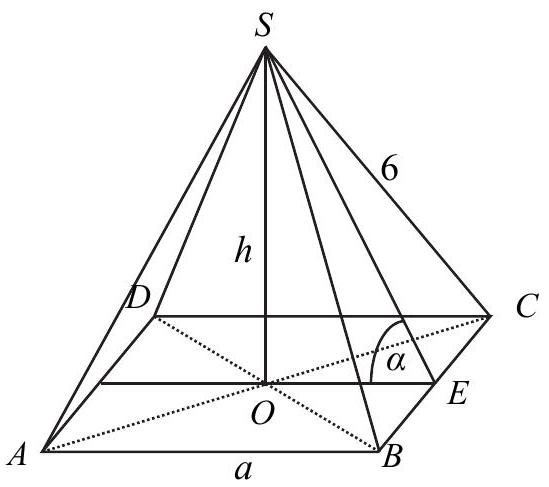
\includegraphics[max width=\textwidth, center]{2025_02_07_d6086222b99967346d9dg-35}

Korzystając z definicji tangensa kąta ostrego w trójkącie prostokątnym SOE otrzymujemy związek $\frac{h}{\frac{1}{2} a}=\sqrt{7}$, czyli $h=\frac{\sqrt{7}}{2} a$.\\
Z twierdzenia Pitagorasa w trójkącie SOC wynika równanie $h^{2}+\left(\frac{a \sqrt{2}}{2}\right)^{2}=6^{2}$.\\
Wykorzystując wcześniejszą zależność otrzymujemy

$$
\left(\frac{\sqrt{7}}{2} a\right)^{2}+\left(\frac{a \sqrt{2}}{2}\right)^{2}=6^{2}
$$

$$
\begin{gathered}
\frac{7}{4} a^{2}+\frac{2}{4} a^{2}=36 \\
\frac{9}{4} a^{2}=36, \text { stąd } a^{2}=16, \text { czyli } a=4 .
\end{gathered}
$$

Stąd $h=4 \cdot \frac{\sqrt{7}}{2}=2 \sqrt{7}$. Obliczamy objętość ostrosłupa: $V=\frac{1}{3} \cdot 4^{2} \cdot 2 \sqrt{7}=\frac{32 \sqrt{7}}{3}$.

\section*{Il sposób}
Zaznaczmy na rysunku kąt $\alpha$ - kąt nachylenia ściany bocznej do płaszczyzny podstawy i wprowadzamy następujące oznaczenia:\\
a - krawędź podstawy ostrosłupa, $h$ - wysokość ostrosłupa, $h_{b}$ - wysokość ściany bocznej ostrosłupa\\
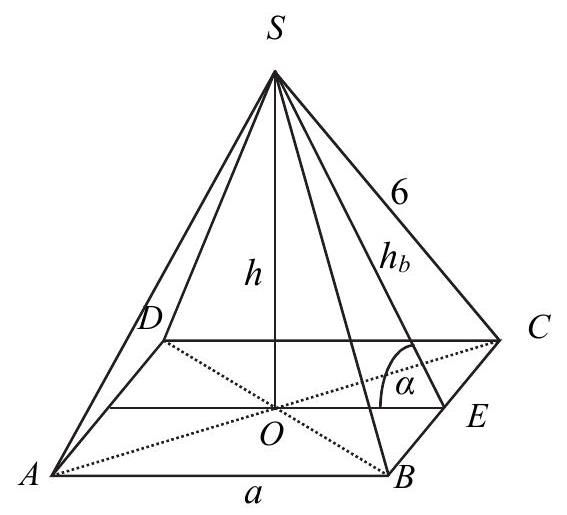
\includegraphics[max width=\textwidth, center]{2025_02_07_d6086222b99967346d9dg-36}

Korzystając z definicji tangensa kąta ostrego w trójkącie prostokątnym SOE otrzymujemy:\\
$\frac{h}{\frac{1}{2} a}=\sqrt{7}$, czyli $h=\frac{\sqrt{7}}{2} a$.\\
Z twierdzenia Pitagorasa w trójkącie prostokątnym SEC otrzymujemy

$$
h_{b}^{2}=6^{2}-\left(\frac{a}{2}\right)^{2}, \quad h_{b}^{2}=\frac{144-a^{2}}{4} .
$$

Z twierdzenia Pitagorasa w trójkącie prostokątnym SOE otrzymujemy

$$
h^{2}+\left(\frac{a}{2}\right)^{2}=h_{b}^{2} .
$$

Zatem

$$
\begin{aligned}
h^{2}+\frac{a^{2}}{4} & =\frac{144-a^{2}}{4}, \\
\frac{7}{4} a^{2}+\frac{a^{2}}{4} & =\frac{144-a^{2}}{4} \\
a^{2} & =16 .
\end{aligned}
$$

Stąd $a=4$, więc $h=2 \sqrt{7}$.\\
Objętość ostrosłupa jest równa: $V=\frac{1}{3} \cdot 4^{2} \cdot 2 \sqrt{7}=\frac{32}{3} \sqrt{7}$.

\section*{Uwaga}
Zależności między wielkościami $h$, a i $h_{b}$ możemy też otrzymać, wykorzystując definicje funkcji sinus lub cosinus kąta $\alpha$. Jeżelitg $\alpha=\sqrt{7}$, to $\sin \alpha=\frac{\sqrt{14}}{4}$ i $\cos \alpha=\frac{\sqrt{2}}{4}$. Stąd $\frac{h}{h_{b}}=\frac{\sqrt{14}}{4}$ oraz $\frac{\frac{1}{2} a}{h_{b}}=\frac{\sqrt{2}}{4}$.

\section*{Ocena prac osób ze stwierdzona dyskalkulia}
Obowiązują zasady oceniania stosowane przy sprawdzaniu prac zdających bez stwierdzonej dyskalkulii z dodatkowym uwzględnieniem:\\
I. ogólnych zasad oceniania zadań otwartych w przypadku arkuszy osób ze stwierdzoną dyskalkulią (punkty 1.-12.);\\
II. dodatkowych szczegółowych zasad oceniania zadań otwartych w przypadku arkuszy osób ze stwierdzoną dyskalkulią - matura z matematyki, poziom podstawowy, termin główny 2020.

\section*{I. Ogólne zasady oceniania zadań otwartych w przypadku arkuszy osób ze}
 stwierdzona dyskalkulia\begin{enumerate}
  \item Nie należy traktować jako błędy merytoryczne pomyłek, wynikających z:
\end{enumerate}

\begin{itemize}
  \item błędnego przepisania,
  \item przestawienia cyfr,
  \item zapisania innej cyfry, ale o podobnym wyglądzie,
  \item przestawienia położenia przecinka.
\end{itemize}

\begin{enumerate}
  \setcounter{enumi}{1}
  \item W przypadku błędów, wynikających ze zmiany znaku liczby, należy w każdym zadaniu oddzielnie przeanalizować, czy zdający opanował inne umiejętności, poza umiejętnościami rachunkowymi, oceniane wzadaniu. W przypadku opanowania badanych umiejętności zdający powinien otrzymać przynajmniej 1 punkt.
  \item We wszystkich zadaniach otwartych, w których wskazano poprawną metodę rozwiązania, części lub całości zadania, zdającemu należy przyznać przynajmniej 1 punkt, zgodnie z kryteriami do poszczególnych zadań.
  \item Jeśli zdający przedstawia nieprecyzyjne zapisy, na przykład pomija nawiasy lub zapisuje nawiasy $w$ niewłaściwych miejscach, ale przeprowadza poprawne rozumowanie lub stosuje właściwą strategię, to może otrzymać przynajmniej 1 punkt za rozwiązanie zadania.
  \item W przypadku zadania wymagającego wyznaczenia pierwiastków trójmianu kwadratowego zdający może otrzymać 1 punkt, jeżeli przedstawi poprawną metodę wyznaczania pierwiastków trójmianu kwadratowego, przy podanych w treści zadania wartościach liczbowych.
  \item W przypadku zadania wymagającego rozwiązania nierówności kwadratowej zdający może otrzymać 1 punkt, jeżeli stosuje poprawny algorytm rozwiązywania nierówności kwadratowej, przy podanych w treści zadania wartościach liczbowych.
  \item W przypadku zadania wymagającego stosowania własności funkcji kwadratowej zdający może otrzymać 1 punkt za wykorzystanie konkretnych własności funkcji kwadratowej, istotnych przy poszukiwaniu rozwiązania.
  \item W przypadku zadania wymagającego zastosowania własności ciągów arytmetycznych lub geometrycznych zdający może otrzymać 1 punkt, jeżeli przedstawi wykorzystanie takiej własności ciągu, która umożliwia znalezienie rozwiązania zadania.
  \item W przypadku zadania wymagającego analizowania figur geometrycznych na płaszczyźnie kartezjańskiej zdający może otrzymać punkty, jeżeli przy poszukiwaniu rozwiązania przedstawi poprawne rozumowanie, wykorzystujące własności figur geometrycznych lub zapisze zależności, pozwalające rozwiązać zadanie.
  \item W przypadku zadania z rachunku prawdopodobieństwa zdający może otrzymać przynajmniej 1 punkt, jeśli przy wyznaczaniu liczby zdarzeń elementarnych sprzyjających rozważanemu zdarzeniu przyjmuje określoną regularność lub podaje prawidłową metodę wyznaczenia tej liczby zdarzeń elementarnych.
  \item W przypadku zadania z geometrii zdający może otrzymać przynajmniej 1 punkt, jeżeli podaje poprawną metodę wyznaczenia długości odcinka potrzebnej do znalezienia rozwiązania.
  \item W przypadku zadania wymagającego przeprowadzenia dowodu (z zakresu algebry lub geometrii), jeśli w przedstawionym rozwiązaniu zdający powoła się na własność, która\\
wyznacza istotny postęp, prowadzący do przeprowadzenia dowodu, to może otrzymać 1 punkt.
\end{enumerate}

\section*{II. Dodatkowe szczegółowe zasady oceniania zadań otwartych w przypadku arkuszy osób ze stwierdzona dyskalkulia}
\section*{Zadanie 26. (0-2)}
Zdający otrzymuje 1 pkt, jeżeli:

\begin{itemize}
  \item w wyniku przekształceń algebraicznych doprowadza nierówność do postaci $a x^{2}+b x+c>0$, gdzie $\Delta>0$ (wystarczy, że z rozwiązania zdającego wynika, że traktuje otrzymaną nierówność jak nierówność kwadratową) oraz stosuje wzory na pierwiastki trójmianu kwadratowego i oblicza te pierwiastki.\\
lub
  \item rozłoży trójmian kwadratowy na czynniki liniowe, z których jednym będzie $(x-1)$\\
lub
  \item poprawnie rozwiąże nierówność $2(x-1)(x+3)>0$.
\end{itemize}

\section*{Zdający otrzymuje 2 pkt, jeżeli:}
\begin{itemize}
  \item Pomyli porządek liczb na osi liczbowej, np. zapisze zbiór rozwiązań nierówności w postaci:
\end{itemize}

$$
(-\infty, 1) \cup\left(-\frac{5}{2},+\infty\right),\left(+\infty,-\frac{5}{2}\right) \cup(1,-\infty)
$$

Uwaga!\\
Jeżeli zdający zapisze zbiór rozwiązań nierówności w postaci sumy przedziałów domkniętych, to może otrzymać co najwyżej 1 pkt.

\section*{Zadanie 27. (0-2)}
\section*{Zdający otrzymuje 1 pkt, jeżeli:}
\begin{itemize}
  \item poda co najmniej dwa poprawne rozwiązania równania.
\end{itemize}

\section*{Zdający otrzymuje 2 pkt, jeżeli:}
\begin{itemize}
  \item przyrówna każdy z czynników do zera, wyznaczy 4 pierwiastki, z których dwa będą prawidłowe (obliczone z jednego czynnika), a w obliczeniu pozostałych pierwiastków będą występowały błędy opisane w pkt 1. i 2. dodatkowych zasad\\
lub
  \item przyrówna każdy z czynników do zera i wyznaczy pierwiastki równania: $x=1, x=0, x=2$ (z pominięciem $x=-1$ ).
\end{itemize}

\section*{Zadanie 28. (0-2)}
\section*{Zdający otrzymuje 1 pkt, jeżeli:}
\begin{itemize}
  \item obliczy wyróżnik trójmianu kwadratowego $a^{2}-2 a b+2 b^{2}$ w zależności od zmiennej $a$ lub $b$
\end{itemize}

\section*{Zdający otrzymuje 2 pkt, jeżeli:}
\begin{itemize}
  \item zapisze nierówność w postaci równoważnej $(a-b)^{2}+b^{2}>0$ oraz stwierdzi (lub zaznaczy), że każdy ze składników lewej strony nierówności jest dodatni.
\end{itemize}

\section*{Zadanie 29. (0-2)}
\section*{Zdający otrzymuje 1 pkt, jeżeli:}
\begin{itemize}
  \item zapisze poprawną proporcję między długościami boków trójkątów $C B D$ i $C E F$, wynikającą z ich podobieństwa np.:
\end{itemize}

$$
\frac{|C F|}{|C E|}=\frac{|C D|}{|C B|}
$$

lub

\begin{itemize}
  \item ustali związki miarowe między długościami boków w jednym z trójkątów prostokątnych $C B D$ lub CEF.
\end{itemize}

\section*{Zadanie 30. (0-2)}
Zdający otrzymuje 1 pkt, jeżeli:

\begin{itemize}
  \item zapisze jedynie liczbę 36 (należy traktować to jako wyznaczenie liczby wszystkich zdarzeń elementarnych)\\
lub
  \item zapisze liczbę 11, a z zapisów wynika, że interpretuje tę liczbę jako liczbę zdarzeń elementarnych sprzyjających zdarzeniu $A$ (np. zilustruje to wypisaniem kilku zdarzeń elementarnych sprzyjających zdarzeniu $A$, ale nie zapisze zdarzeń elementarnych, które nie sprzyjają zdarzeniu $A$ ).
\end{itemize}

\section*{Zdający otrzymuje 2 pkt, jeżeli:}
\begin{itemize}
  \item poprawnie wypisze (lub zaznaczy) wszystkie zdarzenia elementarne sprzyjające zdarzeniu $A$, popełni błąd $w$ ich zliczeniu i konsekwentnie zapisze wynik $\frac{x}{36}$, gdzie $x$ jest liczba zliczonych zdarzeń elementarnych sprzyjających $A$.
\end{itemize}

\section*{Uwaga!}
W ocenie rozwiązania zadania 30. (dla zdających z dyskalkulią) nie stosuje się następującej uwagi z zasad oceniania arkuszy standardowych:

Jeżeli zdający rozwiąże zadanie do końca i otrzyma $P(A)>1$ lub $P(A)<0$, to otrzymuje za całe rozwiązanie 0 punktów, o ile końcowy wynik nie jest skutkiem błędu w działaniach na ułamkach.

\section*{Zadanie 31. (0-2)}
\section*{Zdający otrzymuje 1 pkt, jeżeli:}
\begin{itemize}
  \item doprowadzi równanie $\frac{2 \sin \alpha+3 \cos \alpha}{\cos \alpha}=4$ do postaci $a \sin \alpha=b \cos \alpha$, popełniając ewentualnie błędy opisane w pkt 1. i 2. dodatkowych zasad oceniania\\
lub
  \item poprawnie zastosuje definicje funkcji trygonometrycznych kąta ostrego w trójkącie prostokątnym i poprawnie zapisze równanie $\frac{2 \sin \alpha+3 \cos \alpha}{\cos \alpha}=4 \mathrm{w}$ postaci, w której występują jedynie długości boków trójkąta prostokątnego.
\end{itemize}

\section*{Zdający otrzymuje 2 pkt, jeżeli:}
\begin{itemize}
  \item doprowadzi do równania: $2 \operatorname{tg} \alpha=1$.
\end{itemize}

\section*{Zadanie 32. (0-4)}
\section*{Zdający otrzymuje 1 pkt, jeżeli:}
\begin{itemize}
  \item poprawnie wyznaczy współczynnik kierunkowy prostej $A C$ : $-\frac{3}{4}$.\\
lub
  \item poprawnie zastosuje wzór na odległość punktu $A$ od prostej $B D$.
\end{itemize}

\section*{Zdający otrzymuje 2 pkt, jeżeli:}
\begin{itemize}
  \item zdający wyznaczy poprawne równanie prostej $A C$, zapisuje układ równań, pozwalający obliczyć współrzędne punktu O i rozwiązuje ten układ równań\\
lub
  \item zdający obliczy odległość punktu $A$ od prostej $B D$ i stosuje poprawną metodę obliczenia pola kwadratu, z wykorzystaniem obliczonej odległości.
\end{itemize}

\section*{Zadanie 33. (0-4)}
Stosują się zasady oceniania arkusza standardowego.

\section*{Zadanie 34. (0-5)}
Zdający otrzymuje 1 pkt, jeżeli:

\begin{itemize}
  \item zastosuje poprawnie twierdzenie Pitagorasa dla jednego z trójkątów: SOE lub SEC lub SOC\\
lub
  \item zastosuje poprawnie definicję funkcji tangens w trójkącie SOE dla kąta $\alpha$ :
\end{itemize}

$$
\operatorname{tg} \alpha=\frac{|O S|}{|O E|}
$$


\end{document}